\chapter{Developer documentation}
\label{ch:impl}

\section{Building the code}
\label{sec:building_code}

There are currently two ways of building the code on Windows OS either with Visual Studio and using \textbf{vcpkg} as the package manager or with \textbf{MinGW} and manually building the packages (which I have deprecated but it's possible and I have put it in a separate branch).

First the following steps must be fulfilled to start developing (on windows):

\begin{itemize}
	\item Install \textbf{vcpkg} and add it to your path.
	\item Run the integrate install command so Visual Studio can detect it.
	\item Install CMake.
\end{itemize}

\subsection{Building with CMake}

To make it easier to download the required packages, a powershell script \texttt{install\_dependencies.ps1} is provided with the code which installs all the required dependencies.

Then the project can be built with CMake either by running \texttt{build\_for\_vs.ps1} script or by doing the following in the shell:
\lstset{caption={Building with CMake}, label=src:sh}
\begin{lstlisting}[language=bash]
mkdir build
cd build
cmake .. -G "Visual Studio 17 2022" -A x64 -DCMAKE_TOOLCHAIN_FILE=%PATH_TO_VCPKG%/scripts/buildsystems/vcpkg.cmake
\end{lstlisting}

You can replace generator with your compiler of liking, MinGW, for instance (if you have the packages installed). Replace the tool chain file path to your vcpkg path. 

CMake was chosen because of its cross-platform support. If, for instance, you want to build on linux and have the required packages then you can build using the same CMake file, in which case it will generate a Makefile instead of the VS solution.

\section{Design and the rendering pipeline}
This sections describes how the components fit together and in what order the things are rendered before proceeding to explain all steps in detail.

\subsection{The OpenGL Rendering Pipeline}
\begin{figure}[H]
    \centering
    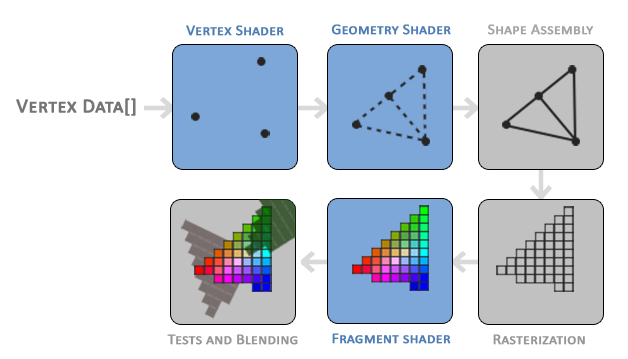
\includegraphics[width=0.75\textwidth]{images/opengl_pipeline.png}
    \caption{The OpenGL Pipeline} \cite{learnopengl}
    \label{fig:opengl_pipeline}
\end{figure}

First let's look at the OpenGL rendering pipeline in Figure~\ref{fig:opengl_pipeline}. The only procedures that we are concerned with at the moment are Vertex and Fragment shaders. Geometry shaders will be described at a later stage when they are needed.

\begin{definition}{Shaders}
	Shaders are programs that run on the GPU, there are various ways to send data to shaders. In the code, I mainly send data through vertex buffers or through uniforms. 
\end{definition}

Without going into too much depth, vertex shaders transform vertices from local space to normalized device coordinates and fragment shaders are used for choosing the colors (as depicted in the picture above).

\subsection{Vertex Shader Convention}
The code snippet below describes how a typical vertex shader looks like in the code:
\lstset{caption={Vertex shader convention}, label=src:vertex_convention}
\begin{lstlisting}[language=C]
layout (location = 0) in vec3 aPos;

uniform mat4 proj;
uniform mat4 view;
uniform mat4 model;

void main() {
	gl_Position = proj * view * model * vec4(aPos, 1.0);
}

\end{lstlisting}

In this document, I will be representing the projection matrix as $\mathbf{P}$, view as $\mathbf{V}$, and model as $\mathbf{M}$. In some vertex shaders there is also a local transformation matrix because I sometimes like to dissect the model matrix into two matrices the model and the local matrix, the former puts the object into the world space and the local transformation is responsible for any rotation or scaling.

\subsection{Shader loader}
To make it easier to load, compile and use shaders the engine comes with a Shader loading
class. The design of the shader loader/manager is inspired by the one on LearnOpenGL \cite{learnopengl}. This class is responsible for allocating and destructing the shaders. A different class is also defined specifically for loading Compute shaders which will be described later. However, the interface for using and setting the uniform variables is identical for both classes.

Uniform variables can easily be set using this shader class, as illustrated in the code snippet below (all such functions can be found in the header file):
\lstset{caption={Shader class usage example}, label=src:shader_usage}
\begin{lstlisting}[language=C++]
Shader myShader {"vertexSource.glsl", "fragmentSource.glsl"};
myShader.use();
myShader.setVec3("cameraPos", glm::vec3(0.0f));
\end{lstlisting}

\subsection{Mesh handling}
\label{subsec:mesh_handling}
In OpenGL the mesh data must be transferred to a \textbf{VBO (Vertex Buffer Object)} first and then the \textbf{VBO} must be bound to a \textbf{VAO (Vertex Array Object)}, instructions for how to parse the data in \textbf{VBO} must also be explicitly defined and optionally a drawing order of vertices can also be defined in a \textbf{EBO (Element Buffer Object)}. To make this simpler a \textbf{Mesh} class comes with the engine. This is also inspired by an implementation on LearnOpenGL \cite{learnopengl}. The figure below gives a rough UML of how the mesh class is structured.

\begin{figure}[H]
    \centering
    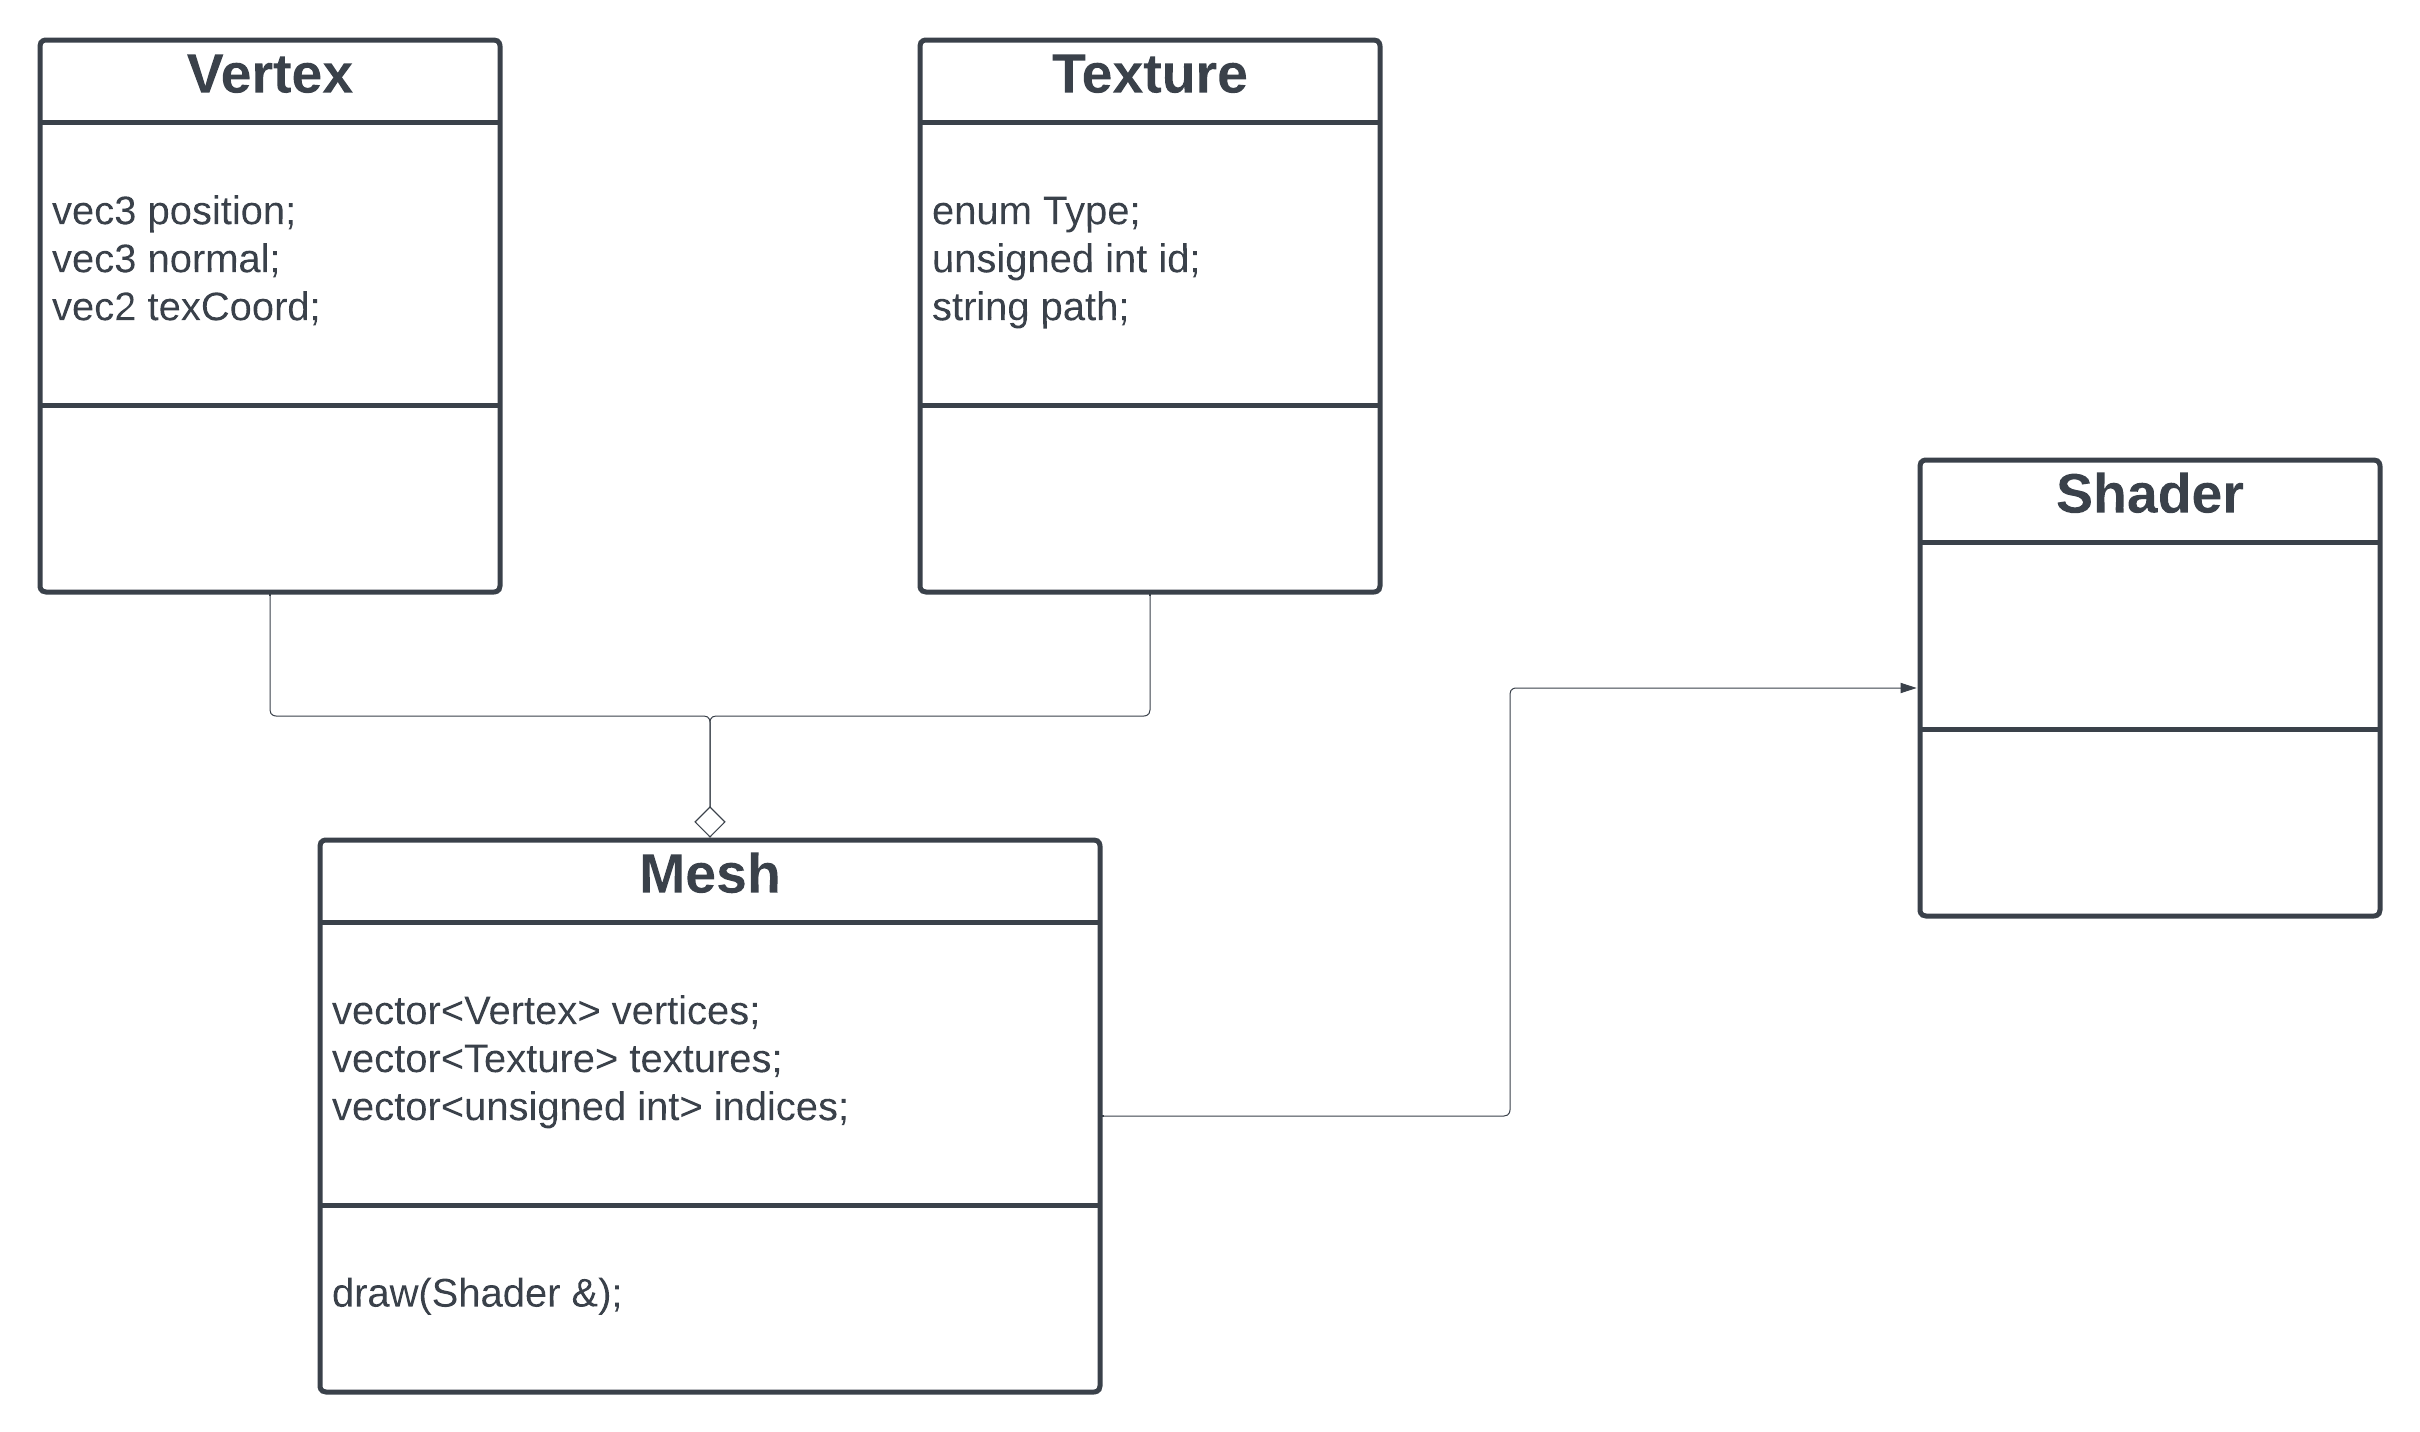
\includegraphics[width=0.75\textwidth]{images/mesh_uml.png}
    \caption{Mesh Class} \cite{learnopengl}
    \label{fig:mesh_uml}
\end{figure}

Meshes for 3d can be generated easily using a mapping $f (u, v)\rightarrow 
\langle x, y, z \rangle$. Some simple examples are given in \texttt{funcs.h} and \texttt{funcs.cpp}. For instance, a sphere can be generated using the function: $f (\theta, \phi) \rightarrow \langle \cos\theta\cos\phi, \sin\phi, \sin\theta\cos\phi \rangle$, where $\theta \in [0, 2\pi], \phi \in [-\frac{\pi}{2}, \frac{\pi}{2}]$. The normal vector for a sphere $\hat{n}$ is, of course, the same as $f (\theta, \phi)$. An implementation for generating the mesh of a torus is also given; a simple version of which can be derived by taking the parametric equation of a circle and translating it along, say, the x axis by $r\prime$: $C (\theta) = \langle r\cos\theta+r\prime, r\sin\theta, 0 \rangle$. If $\mathbf{R_y (\phi)}$ is the rotation around y axis then the torus is $f (\theta, \phi) = \mathbf{R_y( \phi)}C( \theta)$ where $\theta, \phi \in [0, 2\pi]$.


\subsection{Model loading}
The first implementation was done with a custom object file loader, however, it is infeasible to write a complete model loader that triangulates the vertices, supports multiple formats, and pares the texture files accurately. So, the decision to use \textbf{assimp} was made. The \textbf{Model} class is basically a wrapper around \textbf{assimp} functionality. This implementation was also motivated by the one provided on LearnOpenGL \cite{learnopengl}, however, contrary to that implementation this one is more optimized and handles the loading of materials more accurately.

The figure below can be used as a reference for understanding the code in the Model class.
\begin{figure}[H]
    \centering
    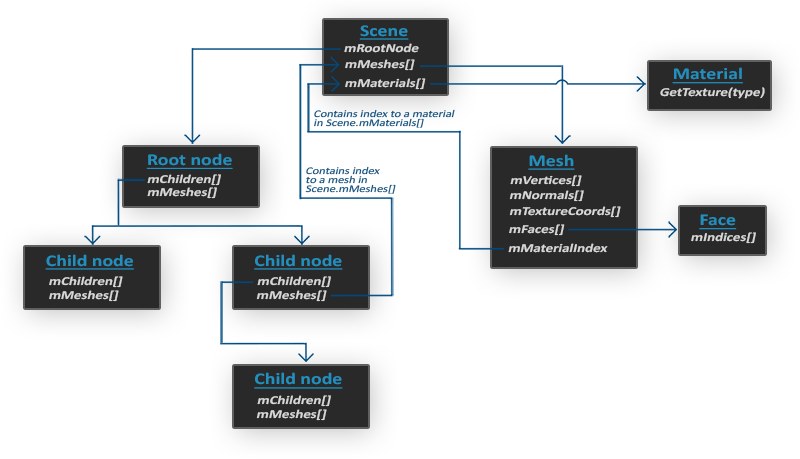
\includegraphics[width=0.75\textwidth]{images/assimp_structure.png}
    \caption{Assimp Structure} \cite{learnopengl}
    \label{fig:assimp_structure}
\end{figure}

A model can be thought of as a collection of meshes, so the rough UML diagram of the class below should make sense:
\begin{figure}[H]
    \centering
    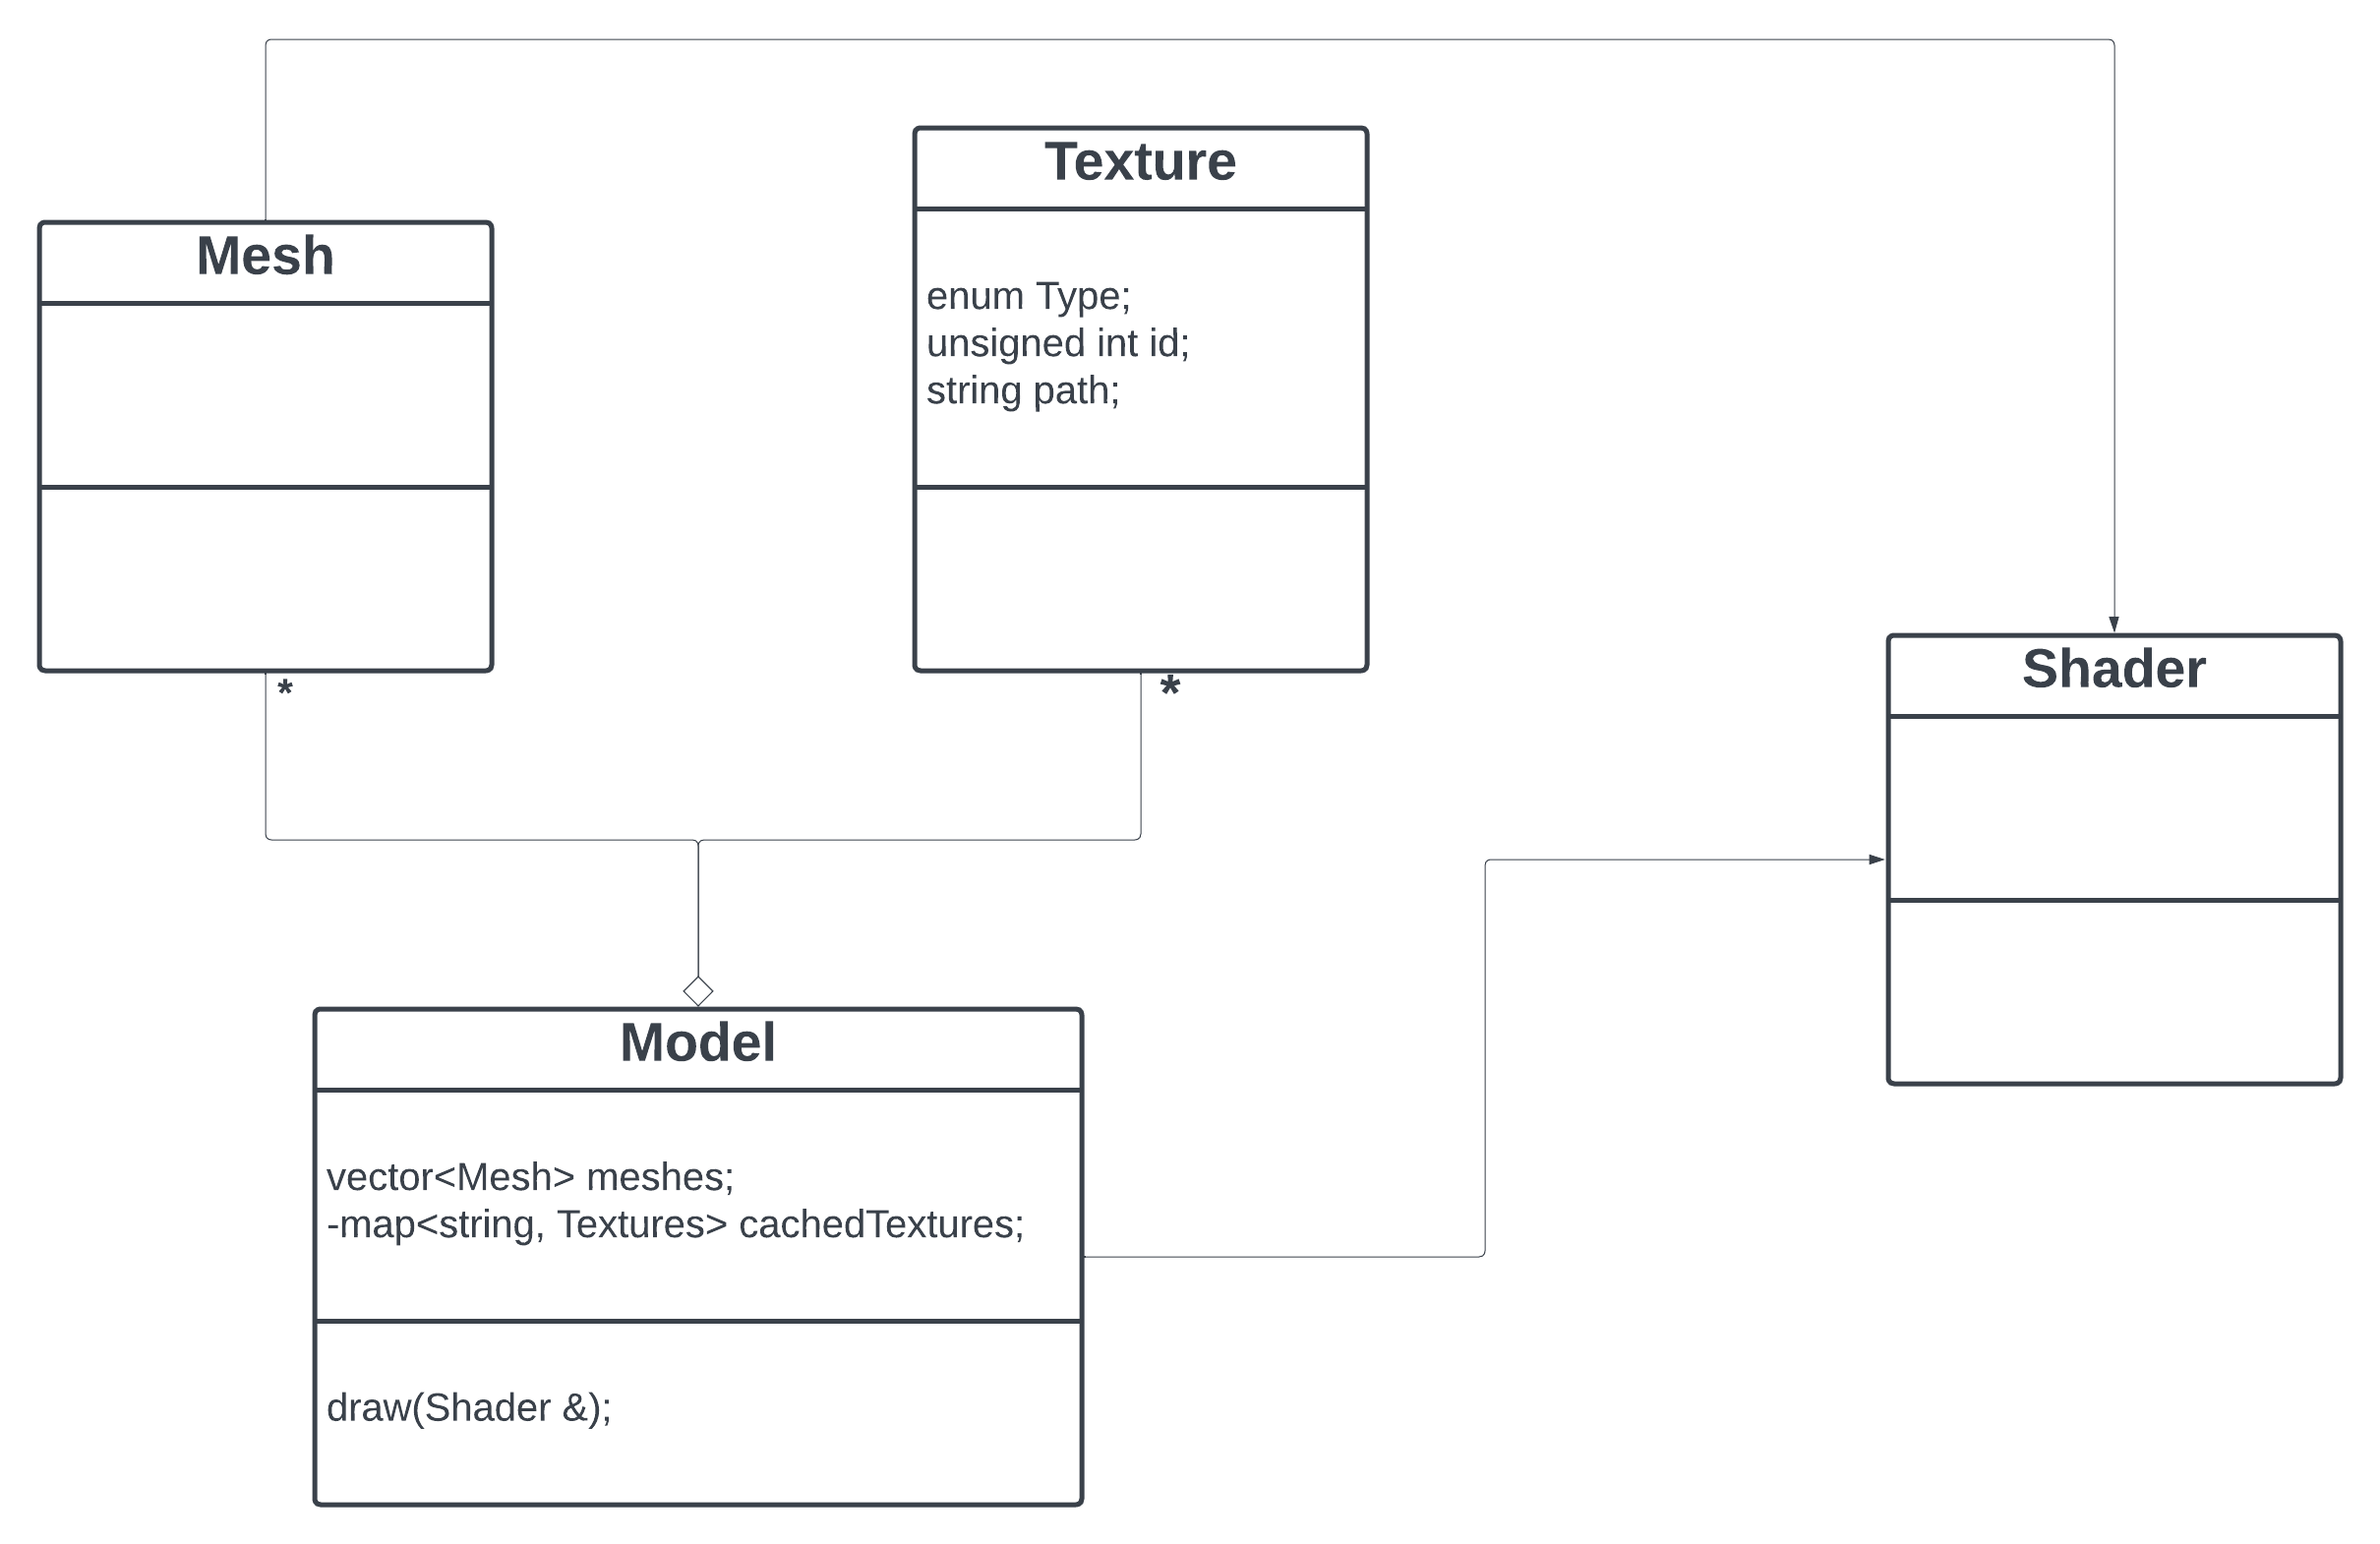
\includegraphics[width=0.5\textwidth]{images/model_uml.png}
    \caption{Model class UML}
    \label{fig:model_uml}
\end{figure}

Since models can have multiple diffuse and specular textures, they must be defined in the shaders in following convention. Diffuse textures must follow the following naming \textbf{texture\_diffuse[1..]}, specular textures must be named as \textbf{texture\_specular[1..]}.


\subsection{\texttt{Camera} class and the camera transform}

\begin{figure}[H]
    \centering
    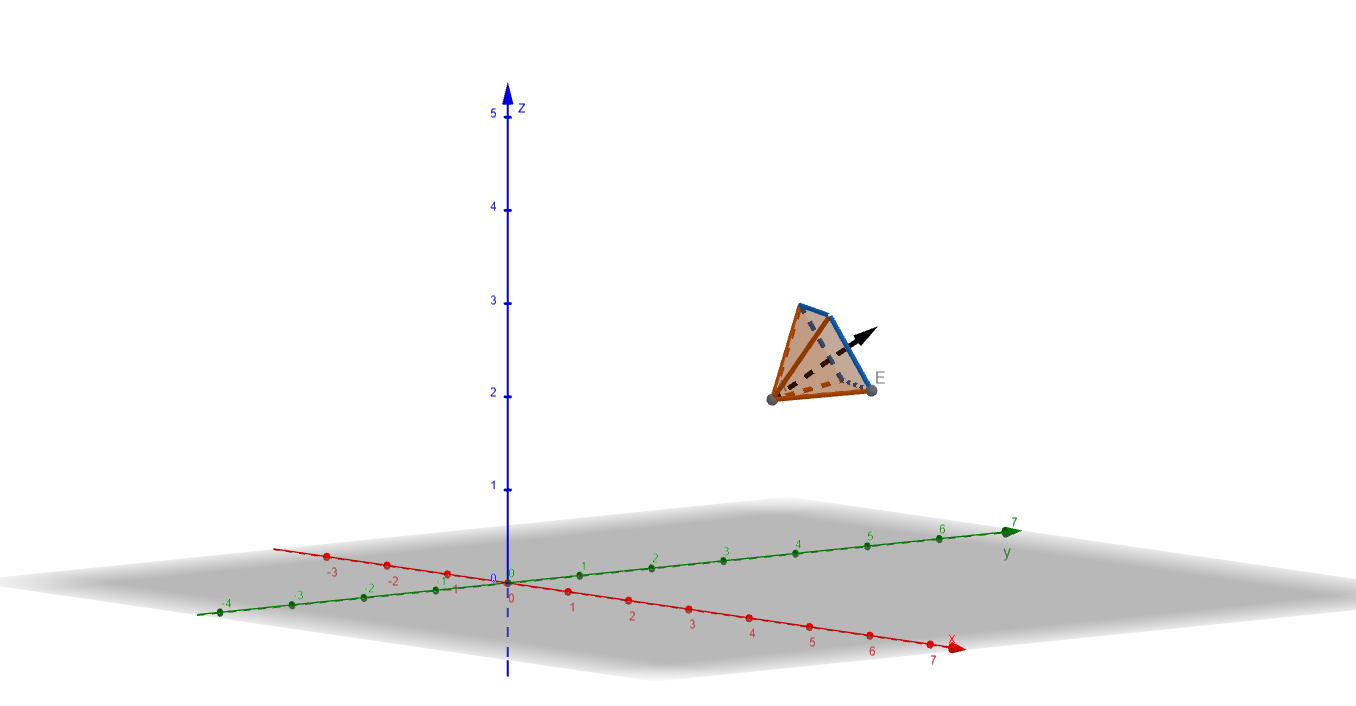
\includegraphics[width=0.75\textwidth]{images/camera_eg2.png}
    \caption{Simple Camera example}
    \label{fig:camera_eg}
\end{figure}

The camera can be imagined as a vector in the figure above. It sits at a point $\mathbf{p}$ looking in direction {$\mathbf{\hat{d}}$}. Contrary to some common implementations, which store a lookAt variable to store what point the camera is looking at, I only store the direction which can be dissected into two components: pitch (rotation around the $x-axis$), represented as $\phi$, and yaw (rotation around the $y-axis$) which is represented as $\theta$. Similar to what was done in the meshes section~\ref{subsec:mesh_handling}, it can be observed that these define a spherical coordinate system and we can get $\mathbf{\hat{d}}$ as follows: \begin{equation}\mathbf{\hat{d}} = \langle \cos\theta\cos\phi, \sin\phi, \sin\theta\cos\phi \rangle\end{equation}

However, the pitch is constrained to avoid distortions so, $\phi \in [-\frac{\pi}{4}, \frac{\pi}{4}]$. An absolute up direction vector is also defined for the camera which I will denote as $\hat{u}$ and $\hat{u}=\langle0, 1, 0\rangle$. The projection matrix works by assuming that the camera is looking in the negative $z-axis$ and is sitting at the origin. So $\mathbf{V}$ must be the matrix that puts the camera in this position. $\mathbf{V}$ must first translate the camera to the origin and then apply the inverse rotation of the current camera rotation.

If $\vec{p}$ is the position vector of the camera, then let $\mathbf{T_{-\overrightarrow{p}}}$ represent the translation matrix that translates by $-{\vec{p}}$.


The current rotation matrix of the camera can be obtained by getting the front (but flipped because the camera starts by looking in the negative $z$-axis), right, and up vectors of the camera:

\[
\hat{f} = \text{front} = -\hat{d}
\]
\[
\hat{r} = \text{right} = \hat{d} \times \hat{u}
\]
\[
\hat{a} = \text{up} = \hat{r} \times \hat{d}
\]

The rotation matrix is then:

\[
\mathbf{R} = \begin{bmatrix} 
\hat{r} & \hat{a} & \hat{f} 
\end{bmatrix}
\]

This can be imagined as where the $\hat{i}, \hat{j}, \hat{k}$ vectors land after the transformation.

We want the inverse of this matrix. Since this is an orthonormal matrix, the inverse is the transpose of the matrix:

\[
\mathbf{R^{-1}} = \mathbf{R}^T
\]

Thus, the final view matrix is:

\[
\mathbf{V} = \mathbf{R}^T \mathbf{T}_{-\mathbf{\overrightarrow{p}}}
\]


The \texttt{Camera} class in the code provides the above functionalities, and the view matrix can be easily obtained by calling the \texttt{camera.getView()} method.

\subsection{Audio Manager}

The engine includes an audio manager capable of playing 2D sounds. Currently, there is no implementation available for 3D audio playback. This component serves as a wrapper around the functionality provided by \textbf{OpenAL}. Audio files are loaded using \textbf{libsndfile}, and the engine currently supports only the \textbf{WAV} format.

The following code snippet demonstrates a basic usage example:

\lstset{caption={Audio Manager example}, label=src:audio_manager}
\begin{lstlisting}[language={C++}]
#include <audio_manager.h>
#include <iostream>

int main() 
{
    AudioManager audioMgr;
    audioMgr.play2d("soundfile.wav", /*loop*/ false);
    std::cin.get(); // prevent exiting
}
\end{lstlisting}


% TO DO: add text renderer, sprite renderer, explain homogenous coords if time permits.

\subsection{OpenGL Frame Buffer Objects and the \texttt{FrameBuffer} Class}

OpenGL provides Frame Buffer Objects (FBOs), which can be thought of as off-screen rendering targets—similar to virtual canvases or pseudo-windows that you can draw on. Instead of rendering directly to the screen, FBOs allow rendering to a texture or render buffer. This is particularly useful for post-processing effects, shadow mapping, and deferred rendering techniques.

The \texttt{FrameBuffer} class in the engine serves as a wrapper around OpenGL’s FBO functionality, simplifying the creation, configuration, usage, and memory management of frame buffer objects. It provides functionality to bind the FBO, with the option to clear it upon binding.

For simplicity, this implementation constructs the FBO using textures (rather than \textbf{Renderbuffer Objects}), as most parts of the engine require the ability to read from the framebuffer. A depth buffer is also included. These design choices can be modified in the future to support more flexible configurations.

A simple example is provided below:

\lstset{caption={Frame Buffer example}, label=src:frame_buffer}
\begin{lstlisting}[language={C++}]
#include <framebuffer.h>
#include <iostream>

int main() 
{
    // Ensure OpenGL context is active before using the FrameBuffer
    FrameBuffer frameBuffer;
    frameBuffer.bind();

    // All OpenGL draw calls will now render to the frame buffer
    // ...

    frameBuffer.unBind();

    // Access the color and depth texture IDs if needed
    GLuint colorTex = frameBuffer.textureId;
    GLuint depthTex = frameBuffer.depthTextureId;

    // Or, draw the FBO's content directly to the screen
    frameBuffer.draw(); 
}
\end{lstlisting}


\subsection{Architecture}

The UML diagram below represents a simplified architecture of the whole game and shows how the components connect to each other.

\begin{figure}[H]
    \centering
    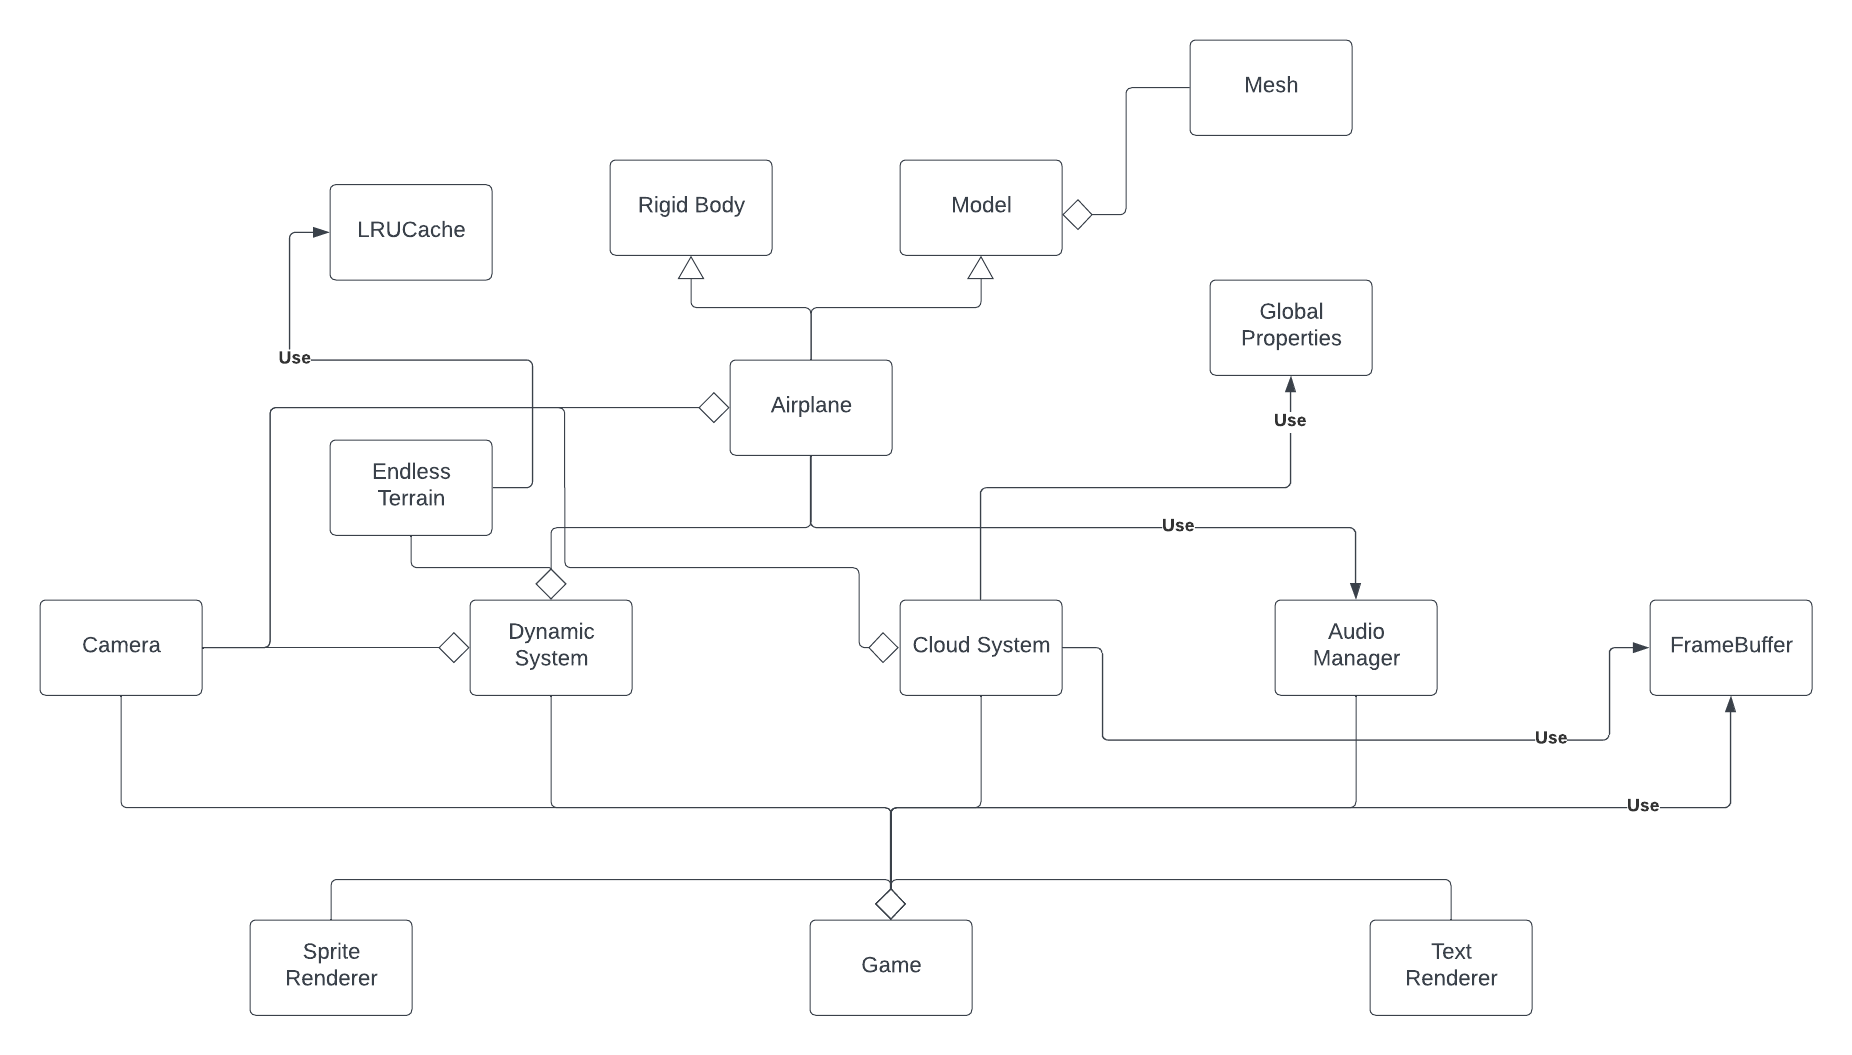
\includegraphics[width=1.0\textwidth]{images/architecture.png}
    \caption{Architecture}
    \label{fig:architecture}
\end{figure}


The main components i.e endless terrain, cloud system, rigid body, and airplane are explained the following sections.

\section{Procedural Terrain}

\subsection{Generating a chunk}

\begin{definition}[Chunk]
A \textit{chunk} refers to a rectangular mesh of predefined size, where each vertex contains height and normal vector information. Chunks serve as the basic building blocks for terrain generation and rendering.
\end{definition}

In most implementations where non-repetitive chunks are required, noise algorithms are commonly used. The algorithm I have chosen is \textbf{Perlin Noise} \cite{perlin2002improving}, which is implemented in \texttt{perlin.cpp}. Assuming, for now that we have some sort of a Perlin noise implementation available, a chunk that only has height data may be generated as simply as the following pseudo code shows:

\lstset{caption={Chunk generation}, label=src:chunk_gen}
\begin{lstlisting}[language=Python]
def generateChunkData(size, scale):
	chunkData = ChunkData(size, size)
	for i in range(size):
		for j in range(size):
			x = j * scale
			y = i * scale
			chunkData.height[i, j] = perlin(x, y)
	return chunkData
\end{lstlisting}

Next, we will explore how to extend this basic chunk with additional data such as normals and how to tile these chunks together for a continuous terrain. We will also dive into techniques such as Level of Detail (LOD) and early culling, which help improve performance and rendering efficiency in large terrains. First, let’s simplify Perlin Noise and look at how to calculate normals for our chunk data.


\subsection{Perlin Noise}

This section does not aim to provide a detailed theoretical explanation of the Perlin Noise algorithm. For a formal treatment, the reader is encouraged to refer to the original paper by Ken Perlin \cite{perlin2002improving}. For a more intuitive and visual explanation, see the video referenced in \cite{perlin_video}. 

Perlin Noise is a type of gradient noise that aims at generating smooth noise. If we, for instance, take a look at white noise where each pixel can be thought of as having a uniform probability of having a value between 0 and 1. The generated map as illustrated in Figure~\ref{fig:white_noise} looks completely random and this would never work as a height map as the height of a terrain is continuous.

\begin{figure}[H]
    \centering
    \begin{minipage}[t]{0.45\textwidth}
        \centering
        
\includegraphics[width=\textwidth]{images/white_noise.png}
        \caption{White Noise}
        \label{fig:white_noise}
    \end{minipage}
    \hfill
    \begin{minipage}[t]{0.45\textwidth}
        \centering
        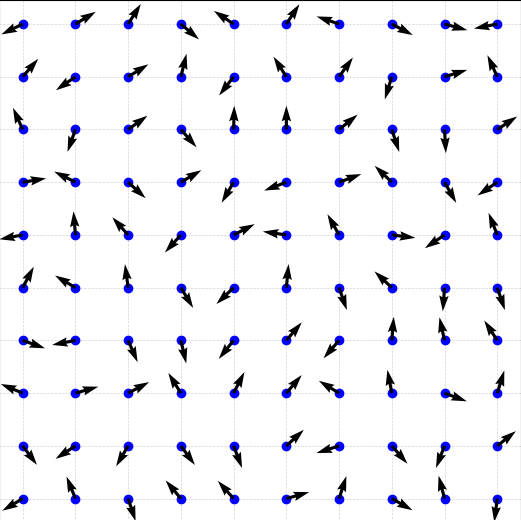
\includegraphics[width=\textwidth]{images/perlin_grid.png}
        \caption{Perlin Grid}
        \label{fig:perlin_grid}
    \end{minipage}
\end{figure}


Before looking into how Perlin noise works, let's define the \texttt{lerp} function.
\begin{definition}[\texttt{lerp}]
	Lerp is defined as :
	\[
		\texttt{lerp}(a, b, p) = a + p(b - a)
	\]
	% lerp(a, b, p) = $a + p(b-a)$
\end{definition}

% Perlin noise works by dividing a plane into a grid that has a random gradient vector assigned at each vertex as shown in Figure~\ref{fig:perlin_grid}. Let's just look at one box and call the point on the top left as $P_{tl}$ and vector associated with as $\vec{v_{tl}}$, we will label other points as $P_{tr}$, $P_{bl}$, $P_{br}$. If we take a point $U$ inside this box with coordinates ($U_x$, $U_y$), and ($u$, $v$) representing the fractional parts of ($U_x$, $U_y$) then the noise function as this point is evaluated as follows:\\
% Let $D_{tl}$ $=$ $P_{tl} - U$, $D_{tr}$, $D_{bl}$, $D_{br}$ are defined similarly. And Let $G_{tl} = \langle V_{tl}, D_{tl} \rangle$, $G_{tr}$, $G_{bl}$, $G_{br}$ are defined similarly.\\
% A step function $g(t)=6t^t-15t^4+10t^3$ is used for smoothing the values of $(u, v)$ and the noise is evaluated as 
% \begin{center}
% 	$noise(U_x, U_y)$ = \texttt{lerp}(\texttt{lerp}($G_{tl}$, $G_{tr}$, $g(u)$), \texttt{lerp}($G_{bl}$, $G_{br}$, $g(u)$), $g(v)$)
% \end{center}

Perlin noise works by dividing the plane into a grid, assigning a random gradient vector at each vertex, as shown in Figure~\ref{fig:perlin_grid}. Consider a single grid cell, and label the corners as follows:
\begin{itemize}
\item{Top-left: $P_{tl}$ with gradient $\vec{v}_{tl}$}
\item{Top-right: $P_{tr}$ with gradient $\vec{v}_{tr}$}
\item{Bottom-left: $P_{bl}$ with gradient $\vec{v}_{bl}$}
\item{Bottom-right: $P_{br}$ with gradient $\vec{v}_{br}$}
\end{itemize}

Let $U = (U_x, U_y)$ be a point inside the cell, and let $(u, v)$ be the fractional parts of $(U_x, U_y)$ relative to the cell.

Define direction vectors from each corner to $U$:
\[
\vec{d_{tl}} = U - P_{tl}, \quad \vec{d_{tr}} = U - P_{tr}, \quad \vec{d_{bl}} = U - P_{bl}, \quad \vec{d_{br}} = U - P_{br}
\]

Next, compute the dot products:
\[
G_{tl} = \langle \vec{v}_{tl}, \vec{d_{tl}} \rangle, \quad G_{tr} = \langle \vec{v}_{tr}, \vec{d_{tr}} \rangle, \quad G_{bl} = \langle \vec{v}_{bl}, \vec{d_{bl}} \rangle, \quad G_{br} = \langle \vec{v}_{br}, \vec{d_{br}} \rangle
\]

A smoothing function is used to interpolate values:
\[
g(t) = 6t^5 - 15t^4 + 10t^3
\]

Finally, the noise value at point $U$ is computed using bilinear interpolation:
\[
\texttt{noise}(U_x, U_y) = \texttt{lerp}(\texttt{lerp}(G_{tl}, G_{tr}, g(u)), \texttt{lerp}(G_{bl}, G_{br}, g(u)), g(v))
\]

\subsection{Calculating normals}
In general, given a parametric surface $f(u, v)$ it is possible to obtain surface normal at specific points by the following formula: 
\[ \hat{n} = \frac{\frac{\partial{f}}{\partial{u}} \times \frac{\partial{f}}{\partial{v}}}
{\|\frac{\partial{f}}{\partial{u}} \times \frac{\partial{f}}{\partial{v}}\|}
\]
One way to imagine this is to see that $\frac{\partial{f}}{\partial{u}}$ and $\frac{\partial{f}}{\partial{v}}$ span the plane that is tangent to the surface, so their cross product gives the normal vector. For a more mathematically sound argument, you can refer to Paul's Online Notes \cite{dawkins_parametric_surfaces}.
In our case the mesh is made up of triangles as seen in Figure~\ref{fig:mesh_eg} but we can still calculate surface normals using cross products.

\begin{figure}[H]
    \centering
    \begin{minipage}[t]{0.45\textwidth}
        \centering
        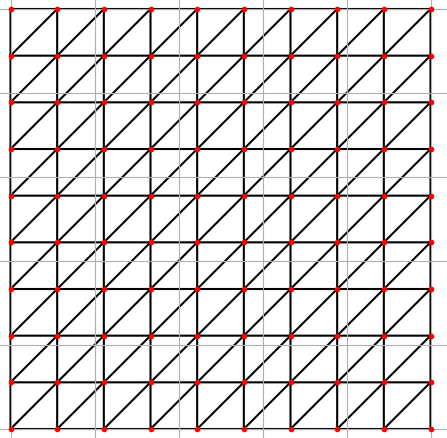
\includegraphics[width=\textwidth]{images/mesh_eg.png}
        \caption{Mesh}
        \label{fig:mesh_eg}
    \end{minipage}
    \hfill
    \begin{minipage}[t]{0.45\textwidth}
        \centering
        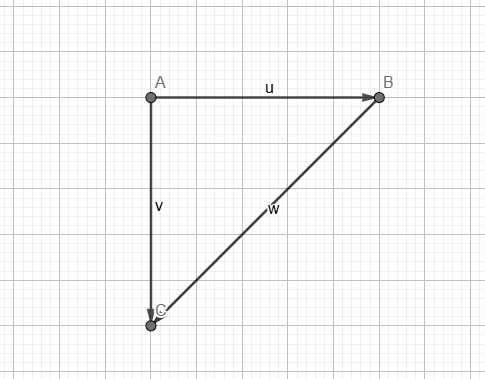
\includegraphics[width=\textwidth]{images/normal_eg.png}
        \caption{Calculating normal of a triangle}
        \label{fig:normal_eg}
    \end{minipage}
\end{figure}

As Figure~\ref{fig:normal_eg} shows we can calculate the normal at vertex \textbf{A} by calculating $u \times v$ (or $v \times u$ this direction is usually checked empirically) where $u$ and $v$ are the vectors of the triangle. This figure is 2d but it can be imagined the all 3 points \textbf{A}, \textbf{B}, and \textbf{C} are at different heights but the math works the same. 

\begin{figure}[H]
    \centering
    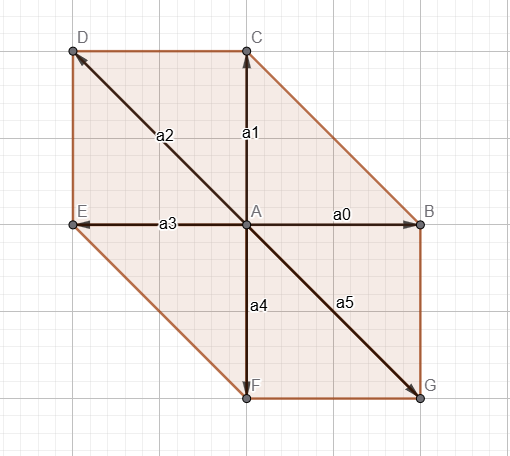
\includegraphics[width=0.5\textwidth]{images/normal_calc.png}
    \caption{Normal Calculation}
    \label{fig:normal_calc}
\end{figure}


However, vertex \textbf{A} is in multiple triangles. Figure~\ref{fig:normal_calc} shows my approach for calculating the normals. I take all the 6 faces (triangles) that vertex \textbf{A} is a part of. Let's call the neighboring vertices of A $\mathbf{N_0}...\mathbf{N_5}$ in either counterclockwise or clockwise ordering (depending on which way defines the cross products in the up direction -- this needs to be checked empirically). Then the normal vector can be calculated as follows:
\[
\vec{n} = \frac{1}{6}\sum_{i=0}^{i=5}{(\mathbf{N_i}-\mathbf{A}) \times (\mathbf{N_{(i+1) \bmod 6}} - \mathbf{A})}
\]
Which is the average of the the normal vectors for each of the 6 triangles. For this to work correctly, you must ensure the vertices are in the correct ordering.

As the picture above suggests, this breaks down at the edges of the mesh. To circumvent this issue, I pad the mesh with extra set of vertices that is used just for the calculation of normals.

So, the pseudocode with normals looks something like this:
\lstset{caption={Chunk generation Part 2}, label=src:chunk_gen2}
\begin{lstlisting}[language=Python]
def generateChunkData(size, scale):
	heightData = Matrix(size + 2, size + 2) // matrix with num rows, cols = size + 2
	for i in range(size + 2):
		for j in range(size + 2):
			x = j * scale
			y = i * scale
			heightData[i, j] = noise(x, y)
	
	chunkData = ChunkData(size, size)
	for i in range(1, size):
		for j in range(1, size):
			vs = getNeighbors(i, j) //should return list of 4  neighbors in the correct order
			vertex = Vector(i, heightData[i, j] ,j)
			normal = Vector(0, 0, 0)
			for k in range(6):
				a = vs[k]
				b = vs[(k + 1) % 6]
				normal += cross(a-vertex, b-vertex)
			mag = normal.magnitude()
			if mag != 0:
				normal /= mag
			chunkData[i-1, j-1].height = heightData[i, j]
			chunkData[i-1, j-1].normal = normal			
	return chunkData
\end{lstlisting}

\subsection{Geometry Shaders and verifying the correctness of the normals}

It still needs to be checked if the normals calculated are actually correct and one way of doing that is to visualize them using geometry shaders. A tutorial for which can be found on LearnOpenGL \cite{learnopengl}. The \texttt{Shader} class provided with the engine takes an optional third argument -the geometry shader source file- so, integrating it into the existing system is easy.  

A geometry shader can take primitives as input (a triangle in our case) and can output primitives. For each vertex of the triangle we can emit a line with two vertices one at the original vertex, the other one in the direction of the normal but scaled by some constant $\alpha$.

The scene must be rendered twice once with the normal shader and again with the geometry shader. Figure~\ref{fig:terrain_normals} was obtained using this pipeline:
\begin{figure}[H]
    \centering
    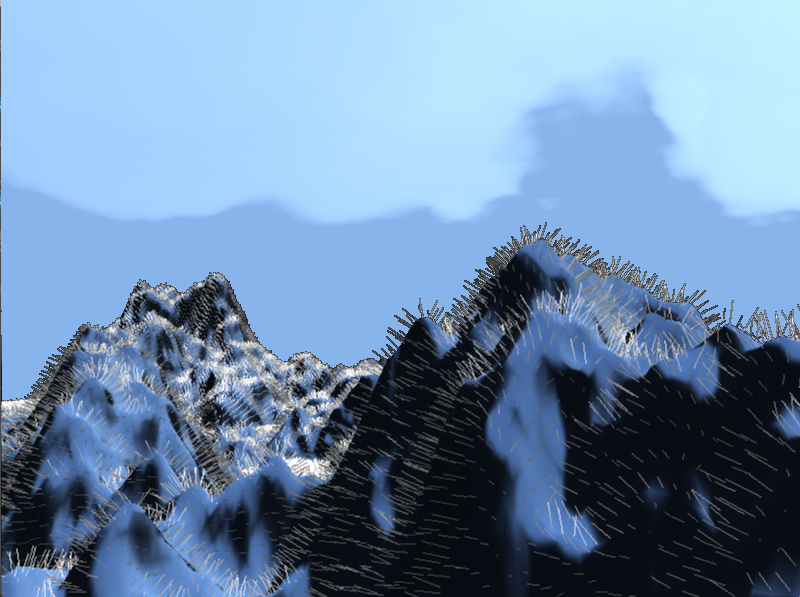
\includegraphics[width=0.5\textwidth]{images/normals.png}
    \caption{Visualizing Terrain Normals}
    \label{fig:terrain_normals}
\end{figure}


\subsection{Tiling the chunks}
Once we have the chunk generation function above it's not too hard to tile them. Since Perlin Noise accepts $(x, y)$ as the arguments we just need to make sure when going from one chunk to the next we give the correct coordinates to Perlin Noise. To do this, I extended the chunk generation function to accept one more argument: its \texttt{center}, using this it calculates the noise as it previously did from its top left corner but this time shifted by the \texttt{center} coordinates.

The following pseudocode explains how it is done:
\lstset{caption={Chunk generation Part 3}, label=src:chunk_gen3}
\begin{lstlisting}[language=Python]
def generateChunkData(size, center, scale):
	heightData = Matrix(size + 2, size + 2) // matrix with num rows, cols = size + 2
	tlX = (size - 1)/-2.0 //top left x
	tlY = (size - 1)/2.0 //top left y
	for i in range(-1, size + 1):
		for j in range(-1, size + 1):
			x = (center.x + tlX + j) * scale
			y = (center.y + tlY - i) * scale
			heightData[i, j] = noise(x, y)
	
	//rest remains same
\end{lstlisting}

If the loop started from \texttt{0}, then \texttt{center.x + tlX} would give the x-coordinate of the current chunk. However, at index $(0, 0)$, we actually want to sample from the previous chunk's coordinate space due to the padding added for normal calculation. Therefore, the loop must begin at \texttt{-1} to correctly align the noise sampling with the padded grid.

\subsection{Level Of Detail (LOD)}

It's important for a better FPS to render the chunks near the player at a higher level of detail than those that are further away. LOD can be thought of in this case as the number of vertices in a given area or volume.

To do this I first create a mesh and then further lower resolution meshes are created by skipping some vertices in the original mesh such that the first and the last vertices are not skipped because the mesh must extend from and to the same points. This begs the question then what should be the size of the original mesh? Consider a 1d mesh of size 10 as the picture below~\ref{fig:one_d} illustrates. We cannot skip every 2nd vertex because then we will have $\langle 0, 2, 4, 6, 8 \rangle$ and the last 9th vertex would be skipped.

\begin{figure}[H]
    \centering
    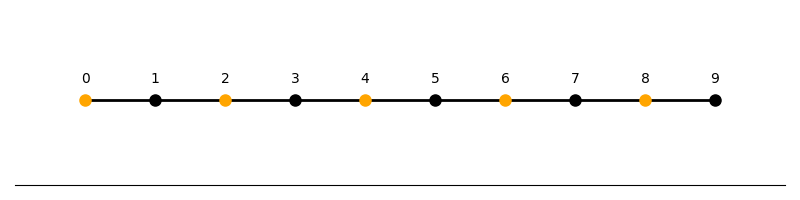
\includegraphics[width=0.75\textwidth]{images/one_d.png}
    \caption{1D mesh}
    \label{fig:one_d}
\end{figure}

So, if $k$ is the skip factor and $s$ is the size of the mesh, then for us to be able to create a mesh, $k$ must divide $s-1$. We need to find $s$ such that $s-1$ has a lot of divisors, and a commonly chosen number is \textbf{$241$} since every number from $1$ to $6$ divides $240$ so we can create a mesh that has $\frac{1}{6}$ of the vertices in the original mesh.

A common approach for this is to generate these meshes on the fly as a function of the distance from the player's coordinates. However, I found this method to not match my FPS goals. So, what I do instead is create the 6 LOD meshes beforehand and give the corresponding mesh its height and normal data through a texture. Height and normal data are stored in a texture, where both of them are packed into a \texttt{vec4} using the red, green, blue, and alpha channels. Each mesh then simply samples from this texture to obtain terrain shape and lighting information.

Unlike traditional LOD systems that generate meshes at runtime based on camera distance, this approach precomputes multiple LOD meshes and uses texture data to drive the final geometry. This reduces runtime computation and improves FPS stability at the cost of some memory overhead.

The image~\ref{fig:lod_terrain} below illustrates how \textbf{LOD} meshes look like in practice.

\begin{figure}[H]
    \centering
    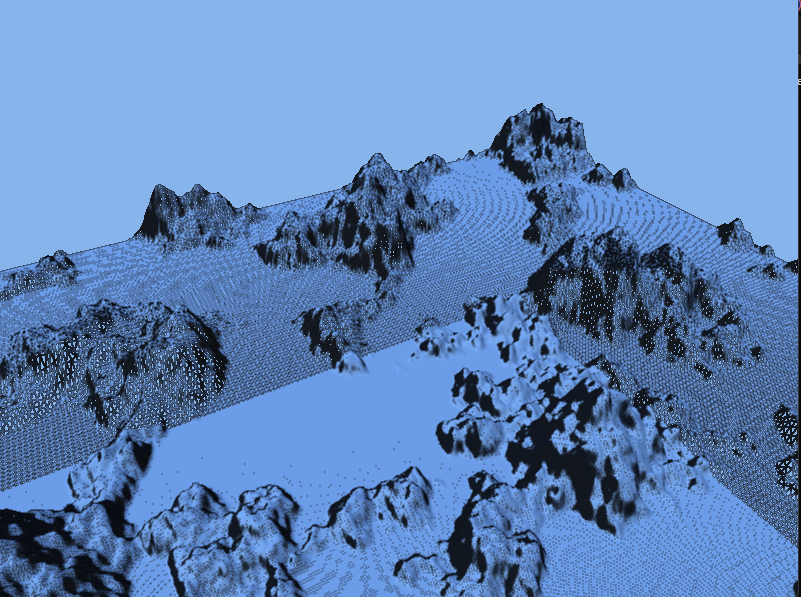
\includegraphics[width=0.5\textwidth]{images/LOD.png}
    \caption{Visualizing LOD Terrain}
    \label{fig:lod_terrain}
\end{figure}

\subsection{Multithreading}
It is not feasible to draw and generate new chunks on the same thread; for instance, we may need to generate 9 chunks at once, which would block the main render loop and drop the frame rate. To avoid this, a new thread is dispatched for generating data for each chunk. Since the meshes are already pre-generated (as discussed in the LOD section), the data needed is just height and normals.
Figure~\ref{fig:chunk_pipeline} illustrates this pipeline.

\begin{figure}[H]
    \centering
    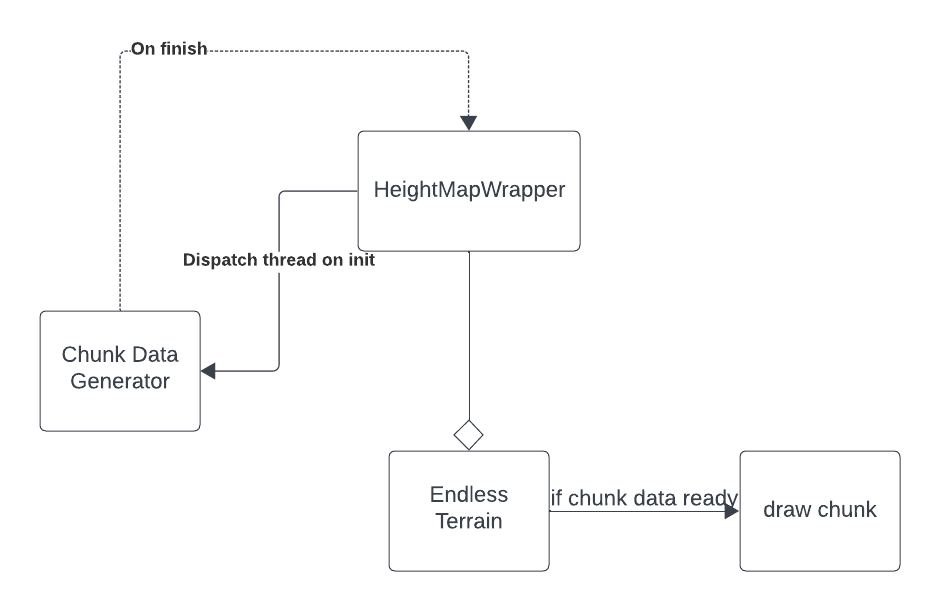
\includegraphics[width=0.75\textwidth]{images/chunk_process.png}
    \caption{Chunk Drawing Pipeline}
    \label{fig:chunk_pipeline}
\end{figure}

The \texttt{EndlessTerrain} class only draws a chunk once its data is ready. When a chunk is needed, it initializes a \texttt{HeightMapWrapper} instance, passing in the chunk center. This wrapper then launches a new thread to request height and normal data from the \texttt{ChunkDataGenerator} (which is just a simple function in the code). Once the data is computed, it is returned via a callback function, completing the pipeline.
\\
\textbf{\large IMPORTANT:}\\
It is crucial to note that OpenGL operates strictly on a single thread—all OpenGL commands must be issued from the same thread that initialized the OpenGL context. Because of this, the \texttt{HeightMapWrapper} class handles all computation on the CPU first. Once the data is available (from the background thread), it schedules OpenGL commands to upload the data to the GPU as a texture, all on the main thread.

\subsection{Caching and the \texttt{LRUCache} class}
Imagine we generate 9 chunks around the player for a single frame, to avoid re-generating them in the next one we must cache them. A straightforward solution would be to use a hashmap where the key is the center of the chunk and the value is the corresponding height map. However, this approach leads to an unbounded cache, which can eventually exhaust system memory.

To solve this, I used the \texttt{LRUCache} class that comes with the engine—a bounded version of the classic hashmap. If the maximum cache size is $n$ and a new key is inserted when the cache is full, the least recently used (LRU) key is evicted to make space.

Since LRUCache is a well-known data structure, its full implementation details are omitted. However, figure~\ref{fig:lru_cache} illustrates its core design using a doubly linked list, which should provide enough insight into how the code operates.

\begin{figure}[H]
    \centering
    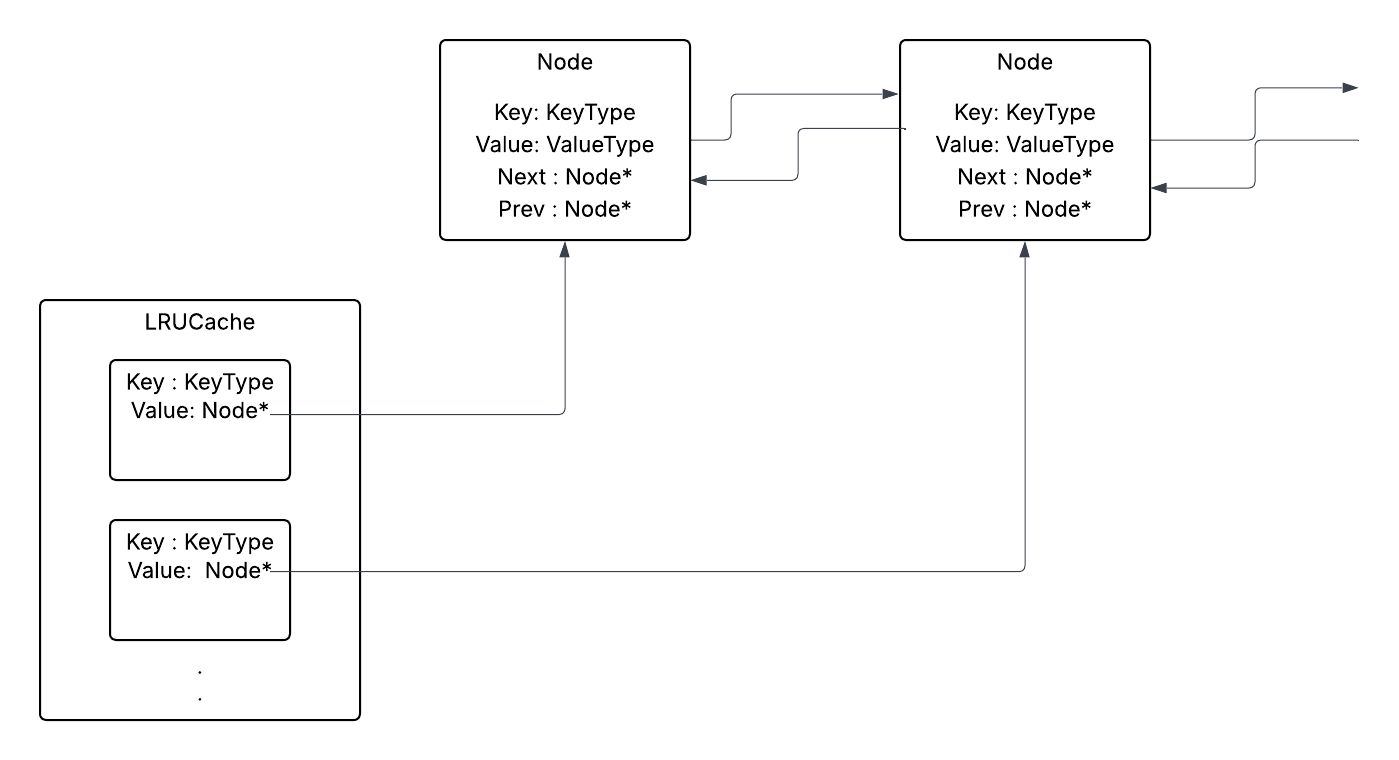
\includegraphics[width=0.75\textwidth]{images/lru_cache.png}
    \caption{LRUCache design}
    \label{fig:lru_cache}
\end{figure}

\subsection{Early Culling}
Notice that the methods above issue generate and draw commands for chunks that are not in the view frustum of the player. This introduces an overhead that can be easily avoided. For instance, the chunks that are behind the player can be omitted. To address this, I use a simple directional culling approach: Say, $\vec{d}$ is the direction of the camera and $\mathbf{P}$ is its position, when we are generating the $i_{th}$ chunk with center $\mathbf{C_i}$ around the player, let $\vec{v} = \mathbf{P}-\mathbf{C_i}$ be the direction of the chunk. We only generate data for the chunk if $\langle \vec{d}, \vec{v} \rangle > 0$ that is, both of those vectors point in the same direction. Note that if $\vec{v}$ is 2 dimensional that $\vec{d}$ must be projected on to the plane. In the code provided, $\mathbf{P}$ is projected onto the $x-z$ plane and so is $\vec{d}$.

\textbf{Result:} This optimization led to a significant performance gain—FPS improved, and memory usage dropped from around 500 MB to around 100MB.


\section{Volumetric Clouds}
This section explains my implementation of volumetric clouds. Before delving into the details, I would like to acknowledge the resources that were instrumental in my work and would like to thank the online community: \cite{sebestianlague2019} \cite{shadertoy2013} \cite{guerrillagames2025nubis} \cite{reinder2018} \cite{fredrik} \cite{gamedevnet2015horizonzerodawn} \cite{palenik2016volumetricclouds} \cite{maxime2023} \cite{engel2016gpupro7}.
\subsection{Ray Marching}

Before rendering clouds, it's essential to understand the basics of ray marching. Ray marching is a technique where we trace rays for each pixel on the screen. Unlike ray tracing, which requires information about polygonal geometry, ray marching only requires access to a signed distance function ($\text{sdf}$). 

A signed distance function for an object $O$ and a point $P$ returns the distance from $P$ to the nearest point on $O$'s surface. It is:
\begin{itemize}
\item{positive if $P$ is outside the object}
\item{negative if $P$ is inside}
\item{and zero if $P$ lies on the surface}
\end{itemize}

For example, the signed distance function for a sphere is:
\[
\text{sdf}(p) = \|p - c\| - r
\]
where $c$ is the center and $r$ is the radius of the sphere.

A ray is defined by its origin $P$ and direction $\vec{d}$. We represent it as a function of time:
\[
R(t) = P + \vec{d}t
\]

If there are multiple objects in the scene, the scene’s overall signed distance function is defined as:
\[
\text{sdf}_{\text{world}}(P) = \min_{\text{objects}} \text{sdf}_{\text{object}}(P)
\]

Ray marching works by advancing the ray by the distance given by the $\text{sdf}$ at each step, as illustrated in the following code snippet:

\lstset{caption={Basic Ray Marching}, label=src:basic_raymarch}
\begin{lstlisting}[language=C]
int MAX_STEPS = 1000;
float MIN_DIST = 1e-4;
float MAX_DIST_TRAVEL = 1e3;

vec3 trace(Ray r) // returns light info
{
    vec3 currentPos = r.pos;
    float totalDistTraveled = 0.0;

    for (int i = 0; i < MAX_STEPS; ++i)
    {
        currentPos = r.pos + r.direction * totalDistTraveled;
        float dist = sdf_world(currentPos);

        if (dist < 0) break;

        else if (dist < MIN_DIST) {
            // do light calculation
            return /* light info */;
        }

        if (totalDistTraveled > MAX_DIST_TRAVEL) break;

        totalDistTraveled += dist;
    }
    return vec3(0.0);
}
\end{lstlisting}

The illustration in Figure~\ref{fig:raymarching_eg} shows this process in 2D, which can be interpreted as a top-down view of a 3D scene.

\begin{figure}[H]
    \centering
    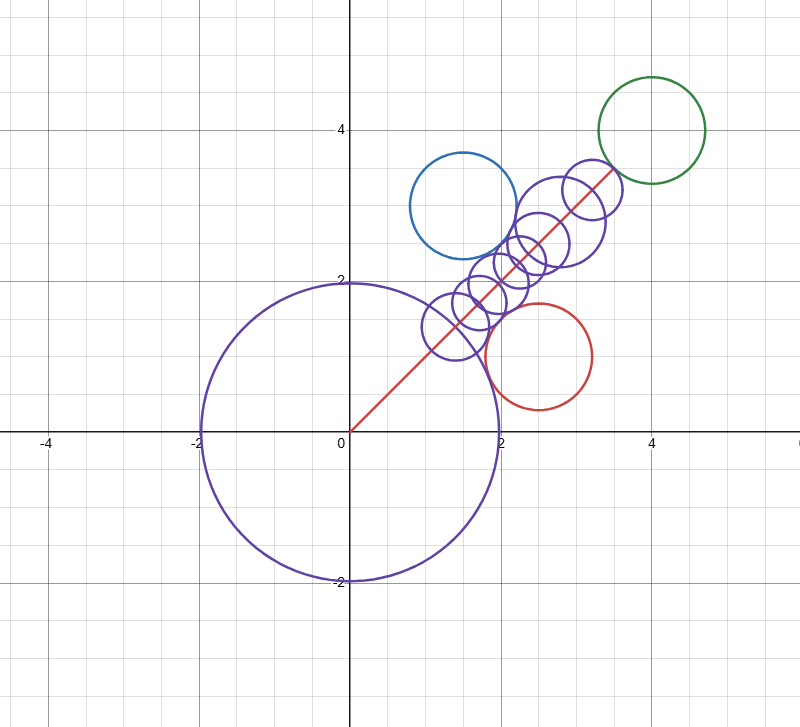
\includegraphics[width=0.5\textwidth]{images/raymarching_eg.png}
    \caption{Ray marching example}
    \label{fig:raymarching_eg}
\end{figure}

When $\text{sdf}(p) = 0$, the surface near point $p$ can be locally approximated by the equation $\text{sdf}(p) = 0$. For an implicit surface $f(x, y, z) = c$ (which can be thought of as a equipotential surface in 3D or level curve in 2D), the surface normal is given by the gradient:
\[
\nabla f = \left\langle \frac{\partial f}{\partial x}, \frac{\partial f}{\partial y}, \frac{\partial f}{\partial z} \right\rangle
\]

Using a symmetric finite difference approximation:
\[
\frac{df}{dx} \approx \frac{f(x + h) - f(x - h)}{2h}
\]

we can approximate the normal at point $p$ from the signed distance function as:
\[
\vec{n} = \left\langle 
\text{sdf}(p + h\hat{i}) - \text{sdf}(p - h\hat{i}),
\text{sdf}(p + h\hat{j}) - \text{sdf}(p - h\hat{j}),
\text{sdf}(p + h\hat{k}) - \text{sdf}(p - h\hat{k})
\right\rangle
\]

This normal vector is then used in lighting calculations.\footnote{This reasoning was derived independently (so it's more intuitive than rigorous) but is consistent with standard SDF-based normal estimation techniques used in ray marching.}

\subsection{Ray Marching for rendering volumes}
For rendering volumetric surfaces like clouds instead of using $sdf$ functions a fixed step size $\delta$ is chosen and the ray is moved forward by this step size at each step. At each point $P$ in space density is sampled and the rendering is done based on how much density was observed, how much light passed through and so on. More details are in the following section but first for clouds my implementation makes a rectangular area in the sky where the clouds can be, this is a axis aligned bounding box (AABB). First, a check is done to see if the ray intersects this box; if yes, only then is the ray marched through the box.
Next, we derive the intersection of a ray with AABB. Remember that a ray is given as $R(T) = P + \vec{d}t$. An axis aligned box can be defined by its top left coordinates and bottom right coordinates denoted as $b_{min}$, $b_{max}$.
\[
b_{min} \le P + \vec{d}t \le b_{max}
\]
\[
b_{min} - P \le \vec{d}t \le b_{max} - P
\]
which gives 3 inequalities:
\[
\frac{(b_{min, x} - P_x)}{\vec{d}_x} \le t \le \frac{(b_{max, x} - P_x)}{\vec{d}_x}
\]
\[
\frac{(b_{min, y} - P_y)}{\vec{d}_y} \le t \le \frac{(b_{max, y} - P_y)}{\vec{d}_y}
\]
\[
\frac{(b_{min, z} - P_z)}{\vec{d}_z} \le t \le \frac{(b_{max, z} - P_z)}{\vec{d}_z}
\]

if $[t_{min}, t_{max}]$ is the intersection of those intervals, then the ray intersects the box if $t_{max} \ge t_{min}$ with $t_{min}$ being the nearest point of intersection and $t_{max}$ being the furthest. If the point is inside the box then clearly, $t_{min} < 0$ in this case we return $t_{max}$ as the intersection $t$. if $t_{max} < 0$, the box must be behind the ray, so there is no intersection.

\subsection{Worley Noise}
Worley noise is a type of cellular noise that we are going to use for generating density textures for clouds. Typically, Worley noise works by choosing $n$ random feature points, in my code I have taken the liberty to call them anchor points. Then for a pixel at location $p$ we calculate its value:
\[
v_p = \min_{anchors} \|p - a_i\| 
\]

$v_p$ for all pixels should be normalized such that $0 \le v_p \le 1$. Figure~\ref{fig:worley_eg} visualizes how this looks like.

\begin{figure}[H]
    \centering
    \begin{minipage}[t]{0.45\textwidth}
        \centering
        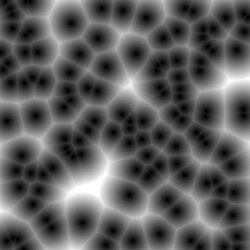
\includegraphics[width=\textwidth]{images/worley.jpg}
        \caption{Worley Noise \cite{wikipedia_worley} }
        \label{fig:worley_eg}
    \end{minipage}
    \hfill
    \begin{minipage}[t]{0.45\textwidth}
        \centering
        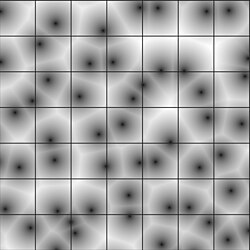
\includegraphics[width=\textwidth]{images/worley_with_grid.jpg}
        \caption{Grid Based Worley Noise \cite{wikipedia_worley}}
        \label{fig:worley_grid}
    \end{minipage}
\end{figure}

However, the naïve approach is computationally expensive, since it requires computing distances from each pixel to all anchor points—scaling poorly as the number of anchors increases. To make it efficient, a grid-based approach is used: the space is divided into regular grid cells, and one anchor point is placed in each cell.

Now, the nearest anchor point for any given pixel can only lie within its own grid cell or one of the adjacent cells. This reduces the number of distance checks significantly.

Normalization becomes straightforward as well: in 2D, the maximum possible distance to a corner in a unit grid cell is $\sqrt{2}$ (assuming the grid cells are of unit area), so the normalized score $s_p$ is:
\[
s_p = \frac{v_p}{\sqrt{2}}
\]
Similarly, in 3D, the normalization factor becomes $\sqrt{3}$:
\[
s_p = \frac{v_p}{\sqrt{3}}
\]

A more useful version in our case is \textbf{Inverted Worley Noise} which is calculated as $1 - s_p$. This gives the bubbly shapes that clouds have as the figure~\ref{fig:inverted_worley} below illustrates:
\begin{figure}[H]
    \centering
    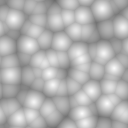
\includegraphics[width=0.5\textwidth]{images/inverted_worley.png}
    \caption{Inverted Worley Noise}
    \label{fig:inverted_worley}
\end{figure}

In the following sections when I say Worley noise, I mean Inverted Worley Noise unless otherwise stated.

\subsection{Making Tileable Worley Noise}
As we will see in the following sections, Inverted Worley noise is used for generating 3D density textures which must be tileable. This means for a pixel on the edge we must take into consideration the cell that is on the other edge (imagine wrapping the grid around like a torus) and the anchor point it contains. My approach for this was to use what I called a deterministic random function which always produces the same value for the same input. The code snippet below shows how it works:
\lstset{caption={Deterministic Random Function}, label=src:det_random}
\begin{lstlisting}[language=Python]
//returns anchor points for grid cell at position pos
def det_random(pos : tuple):
	random.seed(hash(pos))
	return [random.random() for i in range(len(pos))]
\end{lstlisting}

Given some grid coordinates this function generates the anchor point for that cell, even though the anchor point itself is random, it will always give the same anchor point for a given grid cell (in that sense it is deterministic). This way we don't have to store these anchor points. Then we can get the score (or the color) for a pixel as follows:

\lstset{caption={Tileable Worley Noise}, label=src:det_random}
\begin{lstlisting}[language=Python]
//returns anchor points for grid cell at position pos
NUM_TILES  = #number of tiles (boxes)
BOX_WIDTH = WIDTH / NUM_TILES
BOX_HEIGHT = HEIGHT / NUM_TILES
MAX_DIST = sqrt(BOX_WIDTH * BOX_WIDTH + BOX_HEIGHT * BOX_HEIGHT)
def get_color(x, y):
	color = 0.0
	min_d = float('inf')

	#get tile coordinates
	tileX = x // BOX_WIDTH 
	tileY = y // BOX_HEIGHT

	#iterate over neighbor tiles
	for i in range(-1, 2):
		for j in range(-1, 2):
			neighbor_y = (tileY + i) % NUM_TILES 
			neighbor_x = (tileX + j) % NUM_TILES
			anchor_offsetX, anchor_offsetY = det_random((neighbor_x, neighbor_y))

			#rescale to actual coordinates, note these are not wrapped
			anchor_x = (tileX + j + anchor_offsetX) * BOX_WIDTH
			anchor_y = (tileY + i + anchor_offsetY) * BOX_HEIGHT

			min_d = min(min_d, dist((x, y), (anchor_x, anchor_y)))
	color = min_d/MAX_DIST
	#inverted Worley
	return (1 - color)
			
\end{lstlisting}

All textures used in the game were pre generated using Python and the corresponding code can found can be found in the \textbf{\texttt{noise\_scripts}} subdirectory.
\subsection{Fractional Brownian Motion}
Nearly all noise functions used in procedural generation benefit from a technique called \textbf{Fractional Brownian Motion} (fBM). It enhances basic noise by layering multiple octaves—copies of the noise function with increasing frequency and decreasing amplitude—to produce a more complex, self-similar structure reminiscent of fractals. This gives a more natural, detailed appearance when zoomed in.

The following code shows a typical fBM implementation:

\lstset{caption={Fractional Brownian Motion}, label=src:fbm}
\begin{lstlisting}[language=Python]
FREQ_MULT = 2.0
AMPL_MULT = 0.5

def fbm(x, y, octaves):
	ampl = 1 #amplitude
    freq = 1 #fequency
    value = 0.0
    max_val = 0.0
    
    for i in range(octaves):
        value += ampl * noise(x, y)
        max_val += ampl 
        ampl *= AMPL_MULT
        x *= FREQ_MULT
        y *= FREQ_MULT
    
    return value/MAX_NOISE_VAL # normalized
			
\end{lstlisting}

Imagine a plot of a signal, the code above adds higher and higher frequency values of the signal with lower amplitudes to itself to make it appear self-similar.

\subsection{Perlin Worley Noise}
The inverted Worley noise is combined with Perlin noise to add detail to the low-density regions of Perlin noise, creating textures that result in puffier-looking clouds—a technique originating from Guerrilla Games \cite{guerrillagames2025nubis}. Before presenting the formula used to combine the two types of noise, we first define the remap function.
\begin{definition}[Remap function]
    \[\texttt{Remap}(a, old\_min, old\_max, new\_min, new\_max) =\]
    \[new\_min + 
    (new\_max - new\_min)\frac{a-old\_min}{old\_max - old\_min}\]
\end{definition}

Let \( p \) represent Perlin noise and \( w \) the inverted Worley noise. The Perlin-Worley noise is computed as:
\begin{definition}[Perlin Worley Noise]
    \[
    \texttt{PerlinWorley}(p, w)\ = \texttt{remap}(p, 0.0, 1.0, w, 1.0) 
    \]
\end{definition}

The figures below shows how FBM worley noise combined with Perlin noise looks like.

\begin{figure}[H]
    \centering
    \begin{minipage}[t]{0.32\textwidth}
        \centering
        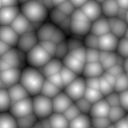
\includegraphics[width=\linewidth]{images/pure_worley.png}
        \caption{Worley Noise}
        \label{fig:pure_worley}
    \end{minipage}
    \hfill
    \begin{minipage}[t]{0.32\textwidth}
        \centering
        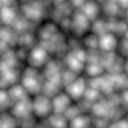
\includegraphics[width=\linewidth]{images/fbm_worley.png}
        \caption{FBM Worley Noise}
        \label{fig:fbm_worley}
    \end{minipage}
    \hfill
    \begin{minipage}[t]{0.32\textwidth}
        \centering
        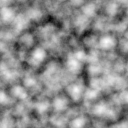
\includegraphics[width=\linewidth]{images/perlin_worley.png}
        \caption{Perlin Worley Noise}
        \label{fig:perlin_worley}
    \end{minipage}
\end{figure}

\subsection{Textures And Sampling Density For Clouds}
One of the 3D textures for clouds contains Perlin-Worley noise in the red channel, and Worley noise of increasing Frequencies in the green, blue, and alpha channels, this is referred to as the low frequency noise texture and its size is $128\times128\times128$. The base cloud is obtained as follows \cite{engel2016gpupro7}:

\lstset{caption={Base Cloud}, label=src:base_cloud}
\begin{lstlisting}[language=Python]
float getCloudDensity(vec3 p)
{
    /*
    normalize p before hand 
    to be able to sample nicely from the texture,
    in the code, this is usually done by multiply 
    p with a uniform scale variable.
    */
    vec4 low_freq = texture(cloudTexture, p);
    float wfbm = 0.625 * low_freq.g + 0.25 * low_freq.b + 0.125 * low_freq.a;
    float baseCloud = Remap(low_frequency_noises.r, wfbm-1.0, 1.0, 0.0, 1.0);

    return baseCloud;

}
\end{lstlisting}

Another 3D texture referred to as high frequency noise texture contains Worley noise of increasing Frequencies, its size is $32\times32\times32$, and this is used for adding details on the edges of the clouds -- this step can be optimized, as we only need to add details to those clouds that are near a certain threshold to the camera.

The last texture that I use is called a weather texture that contains following values \cite{engel2016gpupro7}:
\begin{itemize}
    \item Cloud Coverage: The percentage of cloud coverage in the sky
    \item Precipitation: The chance that clouds will rain (This is not used in my code)
    \item Cloud Type: A value of 0.0 indicates stratus, 0.5 indicates stratocumulus,
    and 1.0 indicates cumulus clouds. 
\end{itemize}


I found the following code snippet on \cite{gamedevnet2015horizonzerodawn} for getting the density of of a cloud based on its type which is given by the weather map:
\lstset{caption={Calculating Specific Cloud Density}, label=src:cloud_density}
\begin{lstlisting}[language=C]

#define STRATUS_GRADIENT vec4(0.0, 0.1, 0.2, 0.3)
#define STRATOCUMULUS_GRADIENT vec4(0.02, 0.2, 0.48, 0.625)
#define CUMULUS_GRADIENT vec4(0.00, 0.1625, 0.88, 0.98)
    
float getDensityForCloudOfType(float heightFraction, float cloudType){
    float stratusFactor = 1.0 - clamp(cloudType * 2.0, 0.0, 1.0);
    float stratoCumulusFactor = 1.0 - abs(cloudType - 0.5) * 2.0;
    float cumulusFactor = clamp(cloudType - 0.5, 0.0, 1.0) * 2.0;

    vec4 baseGradient = stratusFactor * STRATUS_GRADIENT + stratoCumulusFactor * STRATOCUMULUS_GRADIENT + cumulusFactor * CUMULUS_GRADIENT;

    float result = remap(heightFraction, baseGradient.x, baseGradient.y, 0.0, 1.0) * remap(heightFraction, baseGradient.z, baseGradient.w, 1.0, 0.0);
    return result;
}

\end{lstlisting}

To understand what this function is doing, we imagine that the cloudType is $0$, in which case the baseGradient will just be STRATUS\_GRADIENT which defines how the density for the stratus cloud should be. Since stratus clouds are at lower height, the first remap in line $13$ is saying: the density should increase from $0.0$ to $0.1$ height, the second remap is saying: the density should decrease from height $0.2$ to $0.3$, their multiplication gives a gradient (a quadratic function) that is plotted in the image~\ref{fig:stratus_grad} below:
\begin{figure}[H]
    \centering
    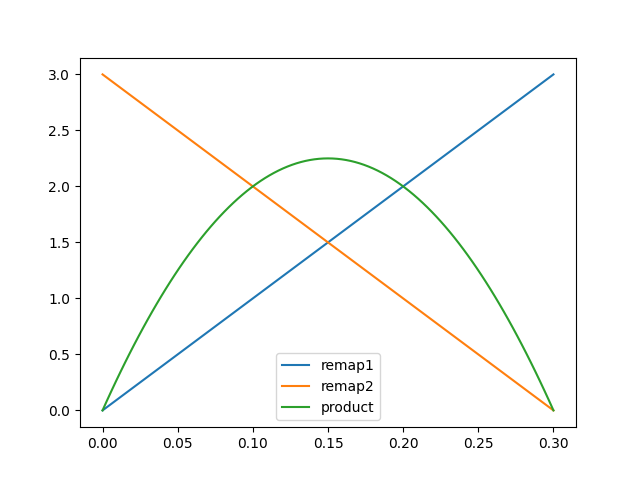
\includegraphics[width=0.5\textwidth]{images/stratus_grad.png}
    \caption{Height Gradient of Stratus Cloud}
    \label{fig:stratus_grad}
\end{figure}

The base cloud above is then enhanced the following way \cite{engel2016gpupro7} \cite{gamedevnet2015horizonzerodawn}:
\lstset{caption={Density For Cloud}, label=src:full_cloud}
\begin{lstlisting}[language=Python]
float getCloudDensity(vec3 p)
{
    /*baseCloud same as above
    boundsMin, boundsMax are the min, max coords of the bounding rectangle (AABB)
    */

    /*this line is not needed if your coverage texture is good enough.*/
    baseCloud = max(baseCloud-densityThreshold, 0.0)

    heightFraction = (p.y - boundsMin.y)/(boundsMax.y-boundsMin.y)
    weatherData = getWeatherTexture(p); //get data from weather texture

    float heightGradient = getDensityForCloudOfType(weatherData.r);
    baseCloud *= heightGradient;

    float coverage = clamp(weatherData.g, 0., 1.) * coverageMultiplier;
    float coverageCloud = remap(baseCloud, coverage, 1., 0., 1.);
    coverageCloud *= coverage;
    float finalCloud = coverageCloud;

    if (finalCloud > 0)
    {
        /*make sure to scale p here too*/
        high_freq = texture(cloudHighTexture, p);
        float highFBM = high_freq.r * .625 + high_freq.g * .25 + high_freq.b * .125;
        /*introduce some height based turbulence*/
        float highModifier = mix(highFBM, 1.0-highFBM, saturate(heightFraction * 10.0));
        /*add details to edges of the cloud (where density is lower)*/
        finalCloud = remap(finalCloud, highModifier*0.2, 1.0, 0.0, 1.0);
    }
    return finalCloud;
}
\end{lstlisting}

\subsection{Lighting}
There is only one light source in the code: the sun. Its direction $\vec{w}_{sun}$ is a global parameter, note that this vector defines direction to the sun and not the other way around. To have accurate lighting for the clouds we need to correctly model how much light they transmit. The most thorough derivations of light calculation I could find were in Juraj Páleník's \cite{palenik2016volumetricclouds} thesis work, \cite{sebestianlague2019} \cite{reinder2018} also seemed to use similar calculations which were instrumental in my understanding of these equations.

When light hits a particle the following things may happen \cite{palenik2016volumetricclouds}:
\begin{itemize}
    \item It may get absorbed by the particle and no longer contribute to lighting effects.
    \item The light may get emitted by matter due to Planck's black body radiation.
    \item The light may get scattered in a different direction.
\end{itemize}

Given a point $x$ and a direction $\vec{w}$, $L(x, \vec{w})$ defines the intensity of the light at point $x$ in the direction $\vec{w}$ (Here $\vec{w}$ is the direction that you shoot your ray in for ray marching). The following differential equation defines the above steps mathematically \cite{palenik2016volumetricclouds}:
\[
    \frac{\partial{L(x, \vec{w})}}{\partial{x}} = -(\alpha(x) + \sigma(x))L(x, \vec{w}) + L_e(x, \vec{w}) + L_i(x, \vec{w}) 
\]

Where $\alpha(x)$ is the light that is absorbed away and $\sigma(x)$ is the light that is scattered, this loss is proportional to how much light there was in the first place. $L_e(x, \vec{w})$ and $L_i(x, \vec{w})$ are the factors for light emitted in at point $x$ in the direction $\vec{w}$ and the light scattered in the direction of $\vec{w}$ which is commonly referred to as in-scattering.

Now, the differential equation above is a first order equation (assuming $\vec{w}$ is constant) and we can put it in the standard form: 
\[
    y' + p(x)y = q(x)
\]
which can be solved using the integral factor: $u=e^{\int{p(x)dx}}$. Let's take $p(x) = (\alpha(x) + \sigma(x))$ and $q(x) = L_e(x, \vec{w}) + L_i(x, \vec{w})$.

We get:
\[
(L(x, \vec{w})e^{\int{p(x)dx}})' = e^{\int{p(x)dx}}q(x)
\]

\[
L(x, \vec{w}) = e^{-\int{p(x)dx}}\int{e^{\int{p(x)dx}}q(x)dx} + Ce^{-\int{p(x)dx}}
\]

If $b$ is the starting point then:
\[
L(a, \vec{w}) = e^{-\int_{b}^{a}{p(x)dx}}\int_b^{a}{e^{\int_x^{a}{p(t)dt}}q(x)dx} + Ce^{-\int_b^{a}{p(x)dx}}
\]

Where $C = L_b = L(b, \vec{w})$. $L_b$ represents the incoming light intensity at the starting point $b$ — for instance, this may be the background color or sky light depending on your implementation.

\[
L(a, \vec{w}) = e^{-\int_{b}^{a}{p(x)dx}}\int_b^{a}{e^{\int_x^{a}{p(t)dt}}q(x)dx} + L_be^{-\int_b^{a}{p(x)dx}}
\]

Rewriting the outer integral to carry out the multiplication:
\[
L(a, \vec{w}) = e^{-\int_{b}^{a}{p(t)dt}}\int_b^{a}{e^{\int_x^{a}{p(t)dt}}q(x)dx} + L_be^{-\int_b^{a}{p(x)dx}}
\]

\[
L(a, \vec{w}) = \int_b^{a}{e^{-\int_{b}^{a}{p(t)dt}+\int_x^{a}{p(t)dt}}q(x)dx} + L_be^{-\int_b^{a}{p(x)dx}}
\]

\[
L(a, \vec{w}) = \int_b^{a}{e^{-\int_{b}^{x}{p(t)dt}}q(x)dx} + L_be^{-\int_b^{a}{p(x)dx}}
\]

Adapting the convention from \cite{palenik2016volumetricclouds}, let $\tau(a, b) = \int_a^b{p(t)dt}$. The equation then becomes: 

\[
L(a, \vec{w}) = \int_b^{a}{e^{-\tau(b, x)}q(x)dx} + L_be^{-\tau(b, a)}
\]

To keep the equations same as in the literature, I will write it as:

\begin{equation}\label{eq:light}
L(a, \vec{w}) = \int_b^{a}{e^{-\tau(x, a)}q(x)dx} + L_be^{-\tau(b, a)}
\end{equation}

which is the same as above but we are integrating $\tau$ in the forward direction in the integral since we start at $b$ and end at $a$.

As noted in \cite{palenik2016volumetricclouds}, the exact form of $L_i$ is the integral of light scattering from all directions (To be precise, this is a surface integral of probability of light scattering times the distribution in which the light scatters in given directions times the intensity of light): 

\[
    L_i(x, \vec{w}) = \frac{1}{4\pi}\int\sigma(x, \vec{w})\tilde{p}(x, w, w')I(x, w, w')d\Omega'
\]

Where $\tilde{p}$ is called the phase function which gives a distribution of redirection of light. Most implementations use the Henyey–Greenstein phase function to model the scattering directionality, which depends on the cosine of the angle between the incoming light direction $\vec{w}_{sun}$ and the viewing direction $\vec{w}$. The exact formula is omitted here as it does not provide significant insight, but it is implemented in the code and widely documented in the literature.

Now we make some simplifications to evaluate this numerically and let's say $\rho(x)$ is the density at point $x$: \cite{palenik2016volumetricclouds}
\begin{itemize}
\item {This was previously mentioned but is worth reiterating: There is only one light source: the sun.}
\item {$L_e(x) = 0$ - there is no emission from the clouds.}
\item {$\alpha(x) = 0$ - no light is absorbed.}
\item {$\sigma(x) = \sigma\rho(x)$} - the light that is scattered away is proportional to the density of the cloud at that point.
\item {$L_i(x, \vec{w}) = \sigma\rho(x)\tilde{p}(\vec{w}.\vec{w}_{sun})e^{-\int_c{\sigma\rho(s)ds}}$} - this is a practical approximation of the in-scattered light. The integral is computed along the ray from point $x$ to the sun and represents the attenuated intensity of sunlight at $x$, according to Beer's law, which states that light intensity decays exponentially as it travels through a participating medium. 
\end{itemize}

Substituting the above simplifications into Equation~\ref{eq:light} we get:
\[
L(a, \vec{w}) = L_be^{-\tau(b, a)} + \int_b^a{e^{-\tau(x, a)}L_i(x, \vec{w})dx}
\]

and 
\[
\tau(a, b) = \int_a^b{\sigma\rho(x)dx}
\]

\[
L(a, \vec{w}) = L_be^{-\tau(b, a)} + \int_b^a{e^{-\tau(x, a)}\sigma\rho(x)\tilde{p}(\vec{w}.\vec{w}_{sun})
e^{-\int_c{\sigma\rho(s)ds}} dx}
\]

Making it discrete, and assuming the integral from $b$ to $a$ is divided into $N$ steps:
\[
L(a, \vec{w}) = L_be^{-T_N} + \sigma\tilde{p}\sum_{i=0}^{N-1}
e^{-T_i}\rho_ie^{-T_i'}\Delta{x}
\]
Where 
\[
T_i = \sum_{j=0}^{i}\sigma\Delta{x}\rho_j
\]
And, 
\[
T_i' = \sigma\Delta{s}\sum_{j=1}^{k}\rho(x + \vec{w}_{sun}j\Delta{s})
\]
which is accumulating the density towards the sun, and in practice $k$ is around 6 as mentioned in \cite{guerrillagames2025nubis}.

\subsection{The Complete Pipeline}
The terrain is rendered first to a framebuffer object (FBO). The cloud rendering pipeline then uses the textures from this FBO as input, layering volumetric clouds on top of the scene — a process commonly known as deferred shading.

A compute shader is used to cast rays from every pixel on the screen. Rays that do not intersect the cloud bounding volume are terminated early for efficiency. For rays that do intersect, the shader performs ray marching through the cloud volume and accumulates light based on the equations discussed previously.

Finally, the result of the compute shader is drawn to the screen.

The figures below show the clouds enclosed within their bounding volume, from both top and bottom perspectives.

\begin{figure}[H]
    \centering
    \begin{minipage}[t]{0.45\textwidth}
        \centering
        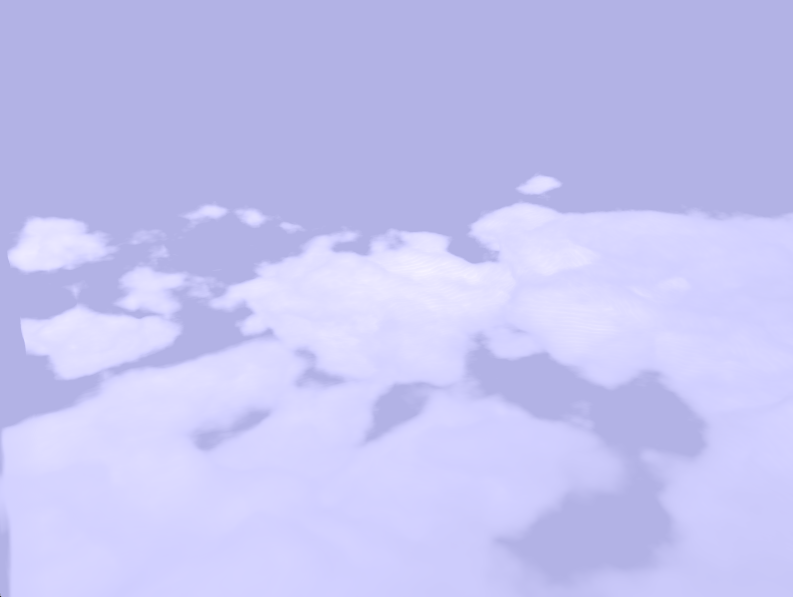
\includegraphics[width=\textwidth]{images/clouds1.png}
        \caption{Clouds top view}
    \end{minipage}
    \hfill
    \begin{minipage}[t]{0.45\textwidth}
        \centering
        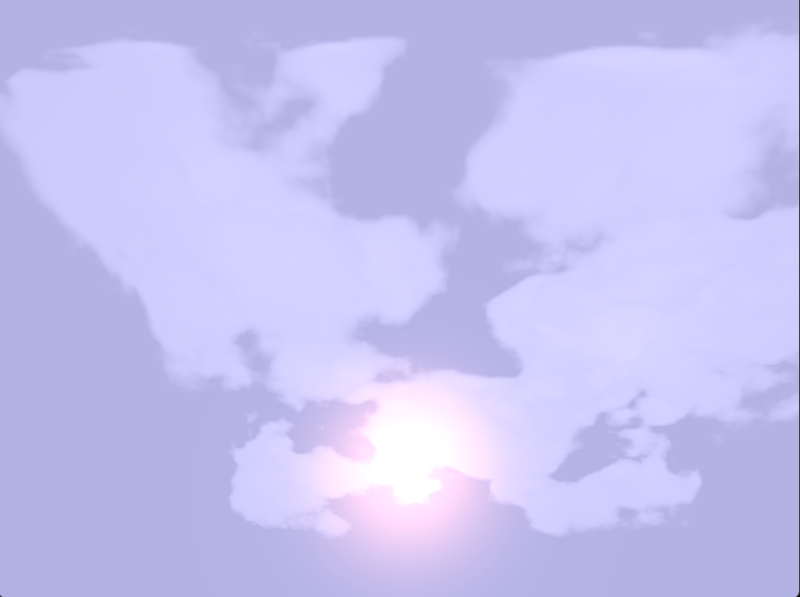
\includegraphics[width=\textwidth]{images/clouds2.png}
        \caption{Clouds bottom view}
    \end{minipage}
\end{figure}

\section{Rigid Body And Airplane}
This section explains my implementation of rigid body and the \texttt{airplane} class with some physics background.

\subsection{Basics}
Given $x(t)$ the position of an object at time t, the velocity is defined as the first derivative of this $v(t) = \dot{x} = \frac{dx}{dt}$ and the acceleration is the derivative of velocity so, $a(t) = \dot{v} = \frac{d^2x}{dt^2}$. We can get position by integrating acceleration as follows: $x = x_0 + v_0t + \frac{a}{2}t^2$. In the code, the rigid body stores the position and the velocity of the body and the updates are performed using euler integration:

\begin{equation}
\label{eq:vel_update}
v_{new} = v_{old} + a\Delta{t}
\end{equation}
\begin{equation}
\label{eq:pos_update}
x_{new} = x_{old} + v\Delta{t}
\end{equation}

But the rigid body has infinite points, which position do we store?

\subsection{Center Of Mass}
Due to Newton's third law which states that: every action has an opposite reaction, we know that the momentum in a closed system is conserved so the force on a object is equal to the external force. If the object is composed of tiny masses $m_i$ at positions $x_i$ we can write this external force as:
\[
F = \sum{m_i\frac{d^2x_i}{dt^2}}
\]
\[
F = \frac{d^2(\sum{m_ix_i})}{dt^2}
\]
If M is the total mass then:
\[
F = M\frac{d^2(\sum{\frac{m_ix_i}{M}})}{dt^2}
\]
\[
F = M\frac{d^2R_{CM}}{dt^2}
\]
Where $R_{CM} = \sum{\frac{m_ix_i}{M}}$ is the center of mass of the rigid body. Since the external force only acts on this point we only need to store this.

\subsection{Linear Force}
When a force $F$ is applied, the acceleration of the rigid body can be calculated as 
\[
a = F/m
\]
This acceleration is then used with equations~\ref{eq:vel_update} and \ref{eq:pos_update} to update the state of the rigid body. Technically, this should be thought of as an impulse which is force applied for time $\Delta t$.

\subsection{Rotational Motion and Torque}

\usetikzlibrary{calc}

\begin{center}
% \begin{tikzpicture}
%   % Original triangle points
%   \coordinate (A) at (0,0);
%   \coordinate (B) at (4,0);
%   \coordinate (C) at (4,3);

%   % Rotate point C around A by dtheta
%   \def\dtheta{10} % degrees
%   \coordinate (D) at ($(A)!1!(C)$); % same as C, for rotation
% %   \path[name path=rotated] (A) -- ($(A)!1!(C)$);
%   \coordinate (D) at ([rotate around={\dtheta:(A)}]C);

%   % Draw original triangle ABC
%   \draw[thick] (A) -- (B) -- (C) -- cycle;
%   \node[below left] at (A) {A};
%   \node[below right] at (B) {B};
%   \node[above right] at (C) {C};

%   % Angle theta
%   \draw[->] (1, 0) arc[start angle=0, end angle=36.87, radius=1cm];
%   \node at (1.2, 0.3) {$\theta$};

%   % Label sides
%   \node at (2, -0.3) {c};
%   \node at (4.3, 1.5) {a};
%   \node at (2.42, 1.45) {r};

%   \draw[->] (1, 0) arc[start angle=36.87, end angle=46.87, radius=1cm];

%   % Draw new triangle ACD
%   \draw[dashed, thick, red] (A) -- (C) -- (D) -- cycle;
%   \node[above right] at (D) {D};

% \end{tikzpicture}

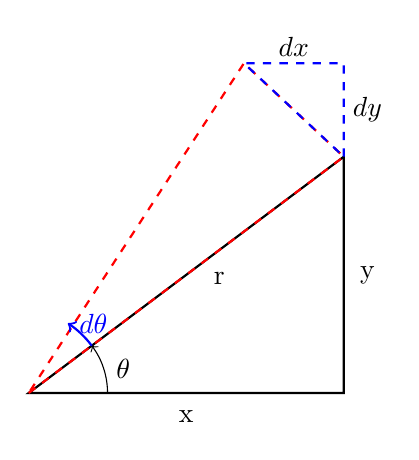
\begin{tikzpicture}
  % Original triangle points
  \coordinate (A) at (0,0);
  \coordinate (B) at (4,0);
  \coordinate (C) at (4,3);
  \coordinate (E) at (4, 4.187);

  % Rotate point C around A by dtheta
  \def\dtheta{20} % degrees
  \coordinate (D) at ([rotate around={\dtheta:(A)}]C);

  % Draw original triangle ABC
  \draw[thick] (A) -- (B) -- (C) -- cycle;
%   \node[below left] at (A) {A};
%   \node[below right] at (B) {B};
%   \node[above right] at (C) {C};

  % Angle theta (angle at A between AB and AC)
  \draw[->] (1, 0) arc[start angle=0, end angle=36.87, radius=1cm];
  \node at (1.2, 0.3) {$\theta$};

  % Label triangle sides
  \node at (2, -0.3) {x};
  \node at (4.3, 1.5) {y};
  \node at (2.42, 1.45) {r};

  \node at (3.366349, 4.4) {$dx$};
  \node at (4.3, 3.5935) {$dy$};

  % Draw new triangle ACD
  \draw[dashed, thick, red] (A) -- (C) -- (D) -- cycle;
%   \node[above right] at (D) {D};

  \draw[dashed, thick, blue] (C) -- (E) -- (D) -- cycle;

  % Draw the small delta-theta arc between AC and AD
  \draw[->, thick, blue] (0.8, 0.6) arc[start angle=36.87, end angle=36.87+\dtheta, radius=1.2cm];
  \node[blue] at (0.82038719, 0.8757653) {$d\theta$};

\end{tikzpicture}
\end{center}

To understand rotational motion take the figure above and imagine the particle is at coordinates $(x, y)$ and is rotated by angle $d\theta$ because of some force. From the picture above it can be seen that $dx = -rd\theta\sin\theta = -rd\theta\frac{y}{r} = -yd\theta$. Similarly, $dy = xd\theta$. From this we get:
\[
\frac{dx}{dt} = v_x = -y\frac{d\theta}{dt} = -y\omega
\]
\[
\frac{dy}{dt} = v_y =  x\frac{d\theta}{dt} = x\omega
\]

Where $\omega=\frac{d\theta}{dt}$ is called the angular velocity. Since $v = \sqrt{v_x^2 + v_y^2}$ is the tangential velocity, we get:
\[
v = \sqrt{y^2\omega^2 + x^2\omega^2} = r\omega
\].

Since work is defined as Force times the displacement, torque is derived from this. Let's look at what the work is in the above equations:

\[ 
W = F_xdx + F_ydy
\]
\[ 
= F_x(-yd\theta) + F_y(xd\theta)
\]
\[ 
= (xF_y - yF_x)d\theta
\]
Work is torque times how much the object rotated. 
\[
\tau = xF_y - yF_x
\]

It can be calculated that this is the derivative of $L = xP_y - yP_x$ which is defined as the angular momentum (where $P$ is the linear momentum). The magnitude of $L$ can be calculated as follows: $L = mv_{\perp}r = mr^2w$. Same as the linear momentum, the term $mr^2$ can be thought of as the hardness to rotate an object, and this is defined as the moment of inertia: $I = mr^2$.

All equations mentioned above have 3D analogues which are more useful to us. Angular velocity can be imagined as a vector that is perpendicular to the plane of rotation.

Torque in 3D is given as: $\tau = r \times F$. The tangential velocity is given as $v = \omega \times r$. The angular momentum is given as: $L = r \times p$ .These can be imagined using the right hand rule for cross products. For a more thorough physics derivation, consult an introductory physics book.

The other more useful representation for $L$ and $\tau$ can be derived as follows:

\[
L = r \times p
\]
\[ 
= r \times mv
\]
\[ 
= mr \times v
\]
\[ 
= mr \times (\omega \times r)
\]
\[ 
= mr \times 
\begin{bmatrix}
    w_yr_z - w_zr_y \\
    w_zr_x - w_xr_z \\
    w_xr_y - w_yr_x  
\end{bmatrix}
\]
\[
= m
\begin{bmatrix}
    r_yw_xr_y - r_yw_yr_x - r_zw_zr_x + r_zw_xr_z \\
    r_zw_yr_z - r_zw_zr_y - r_xw_xr_y + r_xw_yr_x \\
    r_xw_zr_x - r_xw_xr_z - r_yw_yr_z + r_yw_zr_y
\end{bmatrix}
\]
\[
= m
\begin{bmatrix}
    (r_y^2 + r_z^2)w_x - r_yw_yr_x - r_zw_zr_x\\
    -r_xw_xr_y + (r_z^2 + r_x^2)w_y - r_zw_zr_y \\
    -r_xw_xr_z - r_yw_yr_z + (r_x^2 + r_y^2)w_z
\end{bmatrix}
\]
\[
= m
\begin{bmatrix}
    (r_y^2 + r_z^2) && -r_yr_x && -r_zr_x\\
    -r_xr_y && (r_z^2 + r_x^2) && -r_zr_y \\
    -r_xr_z && -r_yr_z && (r_x^2 + r_y^2)
\end{bmatrix}
\begin{bmatrix}
    w_x\\
    w_y\\
    w_z
\end{bmatrix}
\]
\[
= I\omega
\]

Where $I$ is called the inertia tensor. The off diagonal elements are non-intuitive but since this matrix is symmetric, we can diagonalize it so in the eigenbasis the inertia tensor is just a diagonal matrix.

Similarly, torque can be written as:
\[ 
\tau = I\alpha
\]

Where $\alpha$ is the angular acceleration. This equation is the rotational analogue of $F=ma$.

To proceed with rotational updates, we first need to decide how to represent orientation in 3D space.

\subsection{Orientation in 3D and Quaternions}
There are generally three common ways to represent the orientation of a rigid body in 3D. The most well-known method is Euler angles, represented as $(\alpha, \beta, \gamma)$, corresponding to rotations around the $x$, $y$, and $z$ axes. However, this approach is prone to Gimbal lock. Depending on the order in which you apply the rotations, certain configurations can lead to the loss of a degree of freedom. More insights on this can be found in this YouTube video \cite{gimble_video}.

Another method is to represent orientation using a rotation matrix $R$. However, during numerical integration, it's common for the matrix $R$ to lose its orthonormality, requiring periodic re-orthogonalization. Additionally, it requires storing 9 values, which is relatively inefficient.

The most common way of storing orientations in modern physics engines is with quaternions. Quaternions are generalized versions of complex numbers. A quaternion $q$ is represented as:
\[
q = a + bi + cj + dk
\]
where $a$ is called the real part, and $b$, $c$, and $d$ are the imaginary components. If you try really hard, you can imagine this as a unit vector in 4 dimensions.

A video from 3Blue1Brown \cite{3b1b_video} explains how to visualize quaternions in 3D using stereographic projection. Another video \cite{sutrabla_video} explains how they are used for rotations. However, the most rigorous and understandable derivation I could find was in Oleg Viro's lecture notes \cite{viro2016lecture}.

The two representations of quaternions useful for us at the moment are as follows:  
If $q = \cos{\frac{\theta}{2}} + u\sin{\frac{\theta}{2}}$, where $u \in \mathbb{R}^3$ is a unit vector, then the mapping $\mathbb{R}^3 \rightarrow \mathbb{R}^3 : p \rightarrow qp\bar{q}$ describes a rotation of $p$ around the axis $u$ by angle $\theta$.

The other interpretation comes from \cite{sutrabla_video}, where we take a unit quaternion $q = w + xi + yj + zk$ and interpret $w = 1.0$ as no rotation, $x = 1.0$ as a counterclockwise rotation around the $x$-axis, $x = -1.0$ as a clockwise rotation around the $x$-axis, and so on. This interpretation is especially useful in our context, since we use quaternions directly to represent orientation. Remember, these are unit quaternions—so as we adjust $x$ to go from 1.0 to -1.0, the other values must also change accordingly to preserve unit length:
\[
\|q\| = \sqrt{w^2 + x^2 + y^2 + z^2} = 1
\]

Since quaternions are vectors in 4D, using them avoids Gimbal lock entirely. They also make interpolating between two orientations much simpler through SLERP\footnote{Spehrical Linear Interpolation (SLERP) can actually be motivated from complex numbers. If you imagine representing 2D angles as complex numbers, and think about how you would interpolate between two angles, this naturally leads to an explanation for interpolating quaternions. However, this is not directly relevant here, so I decided not to go into it.}. For all these reasons, I chose to use quaternions for rigid body orientation—just like most modern physics engines do.

\subsection{Update equations for rotational motion}
When a torque $\tau$ is applied, we can get the angular acceleration as:
\[
\alpha=I^{-1}\tau
\]
However, this is not quite right, the inertia tensor is defined in the original basis vectors and not the rotated basis vectors (the orientation) of the body. If $R$ is the current orientation of the body then the correct equation is:
\[
\alpha=RI^{-1}R^{-1}\tau
\]
Which can be thought of as follows: transform torque to the original coordinate system, apply inverse inertia tensor transformation, and transform it back to the rotated coordinate system. If $R$ is the matrix of eigenvectors of $I^{-1}$ \footnote{Or eigenvectors of $I$, since $I$ is a symmetric matrix the eigenvectors of $I$ and $I^{-1}$ are the same and the eigenvalues are reciprocals of each other}, then $RI^{-1}R^{-1}$ will be a diagonal matrix (note that $R$ is orthogonal). So, in this situation torque will be in the same direction as the angular acceleration but that is not usually the case.

If $q$ is the current orientation of the body given in quaternions then the updates are done as follows:

\begin{equation}
\label{eq:angvel_update}
\omega_{new} = \omega_{old} + \alpha\Delta{t}
\end{equation}

\begin{equation}
\label{eq:orient_update}
q_{new} = q_{old} + \frac{\Delta{t}}{2}\dot{q}_{old}.q_{old}
\end{equation}
Where 
\[
\dot{q}=0+\dot{q}_xi+\dot{q}_yj+\dot{q}_zk
\]
\[
\dot{q}=0+\omega_xi+\omega_yj+\omega_zk
\]
In other words, $\dot{q}$ is the $\omega$ vector represented as a quaternion.

A derivation of this fact: $\frac{dq(t)}{dt}=\frac{1}{2}\omega(t)q(t)$ can be found in David H. Eberly's Game Physics book \cite{gamephy}.

In practice, $q_{new}$ should also be normalized as it must be a unit quaternion.

\subsection{The \texttt{RigidBody} class}
The \texttt{RigidBody} class in the code encomposses the functionality described above. The methods \texttt{applyTorque}, \texttt{applyForce} behave as you would expect. However, this class also provides \texttt{applyRelativeTorque}, \texttt{applyRelativeForce} methods which apply the provided force relative to the current orientation.
This is supposed to be used with other classes as this by itself has no physical meaning and it represents an abstract body. To be able to draw an object it must inherit from the \texttt{Model} (or \texttt{Mesh}) class and to give it physics properties it must inherit from \texttt{RigidBody} class. Nevertheless, a simple example usage is given below:
\lstset{caption={Rigid Body example}, label=src:rigid_body}
\begin{lstlisting}[language=C++]
#include "rigid_body.h"
#include <glm/glm.hpp>
#include <glm/gtc/matrix_transform.hpp>
#include <glm/gtc/type_ptr.hpp>
#define GLM_ENABLE_EXPERIMENTAL
#include <glm/gtx/quaternion.hpp>

void main(){
    RigidBody obj{/*mass*/ 1.0f, /*pos*/ glm::vec3(0.0f), 
                  /*orient*/ glm::quat(1.0f, 0.0f, 0.0f, 0.0f), 
                  /*inertia tensor*/ glm::mat3(1.0f)};

    obj.applyForce(glm::vec3(2.0f, 0.0f, 0.0f));
    obj.applyRelativeTorque(glm::vec3(1.0f, 0.0f, 0.0f));

    obj.update(0.1f);
}
\end{lstlisting}

\subsection{Airplane}
Normally, when modeling aircraft physics one needs to take into account the lift, drag, and other related forces. For instance, An airplane takes off by generating a pressure difference near the wings, it tilts in a similar fashion with the pressure difference being different for both the wings. However, accurately modeling such phenomena is beyond the scope of this thesis. Instead, I use simplified approximations that strike a balance between physical plausibility and computational efficiency.

\subsection{Estimation of Forces}
\paragraph{Thrust}
Thrust is modeled as a direct force along the aircraft's longitudinal axis, controlled by the throttle input:
\begin{equation}
\vec{F}_{thrust} = \text{throttle} \times \text{maxThrottle} \times \vec{d}_{forward}
\end{equation}

Where $\vec{d}_{forward}$ is the forward direction vector of the aircraft, and throttle is a normalized input value indicated if the forward key was pressed or not.

\paragraph{Control Surface Forces}
Rather than explicitly modeling airflow over control surfaces, the implementation directly maps control inputs to torques:

\begin{equation}
\vec{\tau}_{pitch} = \text{pitchInput} \times \text{pitchSpeed} \times (1 - |\text{currentPitch}|)
\end{equation}

\begin{equation}
\vec{\tau}_{roll} = \text{rollInput} \times \text{rollSpeed}
\end{equation}

\begin{equation}
\vec{\tau}_{yaw} = \text{yawInput} \times \text{yawSpeed}
\end{equation}

The pitch control includes a factor of $(1 - |\text{currentPitch}|)$ which reduces effectiveness at extreme pitch angles, simulating control surface saturation.

\paragraph{Stabilizing Effects}
To simulate natural stability without implementing a full aerodynamic model, corrective torques are applied based on the current orientation:

\begin{equation}
\vec{\tau}_{stabilize\_roll} = -\text{currentRoll} \times \text{stabilizingFactor}
\end{equation}

\begin{equation}
\vec{\tau}_{stabilize\_pitch} = -\text{currentPitch} \times \text{stabilizingFactor}
\end{equation}

These torques tend to restore the aircraft to level flight when no control inputs are applied, approximating the static stability of typical aircraft designs.

\paragraph{Cross-Coupling Effects}
To simulate how real aircraft movements are coupled, additional effects are approximated:

\begin{equation}
\vec{\tau}_{induced\_yaw} = \text{currentRoll} \times \text{inducedYawFactor}
\end{equation}

\begin{equation}
\vec{\tau}_{induced\_pitch} = -|\text{roll}| \times 0.1
\end{equation}

The induced yaw effect simulates the natural tendency of aircraft to yaw in the direction of roll, caused by differential drag on the wings. The induced pitch effect approximates the slight nose-down tendency when banking.

\paragraph{Practical Implementation}
These estimations, while simplified, create a flight model that captures the essential behavior of aircraft without the computational overhead of true aerodynamic simulation. The result is an intuitive flying experience that maintains physical plausibility while being easy to implement and tune.

\begin{lstlisting}[language=C++, caption={Force application in update method}, label=src:force_application]
// Apply thrust
applyRelativeForce(glm::vec3(0.0f, 0.0f, -1.0f) * throttle * maxThrottle);

// Apply combined control torques
applyRelativeTorque(glm::vec3(
    (pitch*(1-std::fabs(currentPitch)) + stabilizingPitch + inducedPitch) * pitchSpeed,
    (yaw + inducedYaw) * yawSpeed,
    (roll*.75+stabilizingRoll*stabilizingRollFactor) * rollSpeed
));
\end{lstlisting}

The simplicity of this approach allows for easy adjustment of flight characteristics through the configuration parameters, making it straightforward to tune the model for different aircraft types or desired handling qualities.


\section{Testing}

\subsection{Building with CMake}
Building with instructions specified in Section~\ref{sec:building_code} does not automatically build tests too. The testing component was seperated for a faster build time.


The instructions specified in Section~\ref{sec:building_code} must be followed as the first step for getting the dependencies then the project with tests can be built with CMake either by running the \texttt{build\_with\_tests.ps1} script (if your vckpg is located in "C:/vckpg") or by doing the following in the shell:
\lstset{caption={Building with CMake}, label=src:sh}
\begin{lstlisting}[language=bash]
mkdir build
cd build
cmake .. -G "Visual Studio 17 2022" -A x64 -DCMAKE_TOOLCHAIN_FILE=%PATH_TO_VCPKG%/scripts/buildsystems/vcpkg.cmake -DBUILD_TESTS=TRUE
\end{lstlisting}

In other words, you can build tests by setting the \texttt{BUILD\_TESTS} flag to true in CMake.

\subsection{Running the tests}
The tests can be run on Visual Studio by navigatings to \texttt{Test}>\texttt{Test Explorer} and clicking on \textbf{Run All Tests In View}. This first builds the code and then discovers the tests, if it does not automatically run the tests navigate to \texttt{Test} and click on \textbf{Run All tests}. The result should look like something show in the figure~\ref{fig:test_results} below.

\begin{figure}[H]
    \centering
    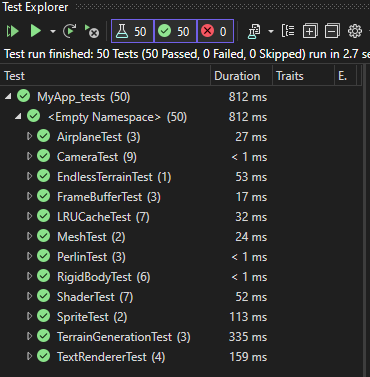
\includegraphics[width=0.75\textwidth]{images/test_results.png}
    \caption{Running the tests in Visual Studio}
    \label{fig:test_results}
\end{figure}

\subsection{Testing Plan}

I decided to use \texttt{Google Test (gtest)} as the testing library because of wide support and easy integration. It's available through vckpg and is installed through the \texttt{install\_dependencies.ps1} script.

The tests are a mixture of unit and integration tests. The components that do not depend on anything else such as LRUCache, PerlinNoise, RigidBody are tested in the style of unit tests. The other components that depend on OpenGL context to be initialized could have followed a similar style, however, for that a lot of classes would have needed be mocked which would have required an implementation of interfaces causing a change to the design of the project. Instead, these tests are done as a hybrid of unit and integration tests and as I'll explain below for the tests that require an OpenGL context, an empty context is built.

\subsection{Unit Tests}
\subsubsection{LRUcache}
LRUCache is an independent component and the following tests were done on it: 
\begin{itemize}
    \item Basic insertion and retrieval functionality
    \item Proper implementation of the LRU eviction policy
    \item Update of access order when elements are accessed
    \item Value overwriting behavior
    \item Size tracking accuracy
    \item Consistent behavior under repeated access patterns
    \item Performance under high-volume operations
\end{itemize}

\subsubsection{Perlin Noise}
The following tests were done for perlin noise:
\begin{itemize}
    \item Consistency: Identical inputs should produce identical outputs
    \item Distinction: Different inputs should produce different outputs
    \item FBM correctness: The multi-octave implementation should match the mathematical definition
\end{itemize}

\subsubsection{Rigid Body}
Following tests were done for rigid body:
\begin{itemize}
    \item Linear movement in response to forces
    \item Damping effects on velocity
    \item Rotation in response to torque
    \item Combined movement from off-center forces
    \item Local vs. global coordinate force application
    \item Orientation normalization under continuous rotation
\end{itemize}

\subsubsection{Camera}
The following tests were implemented for the \texttt{Camera} component:
\begin{itemize}
    \item Initialization: Verifies that a new camera instance is oriented toward the negative Z-axis by default.
    \item Yaw rotation: Confirms that changes in yaw correctly update the front direction vector, including wraparound behavior beyond 360\textdegree.
    \item Pitch clamping: Ensures that pitch values are clamped within a safe range to prevent gimbal lock or distortion.
    \item Movement handling: Tests the camera's response to directional movement commands, updating its position accordingly.
    \item Mouse input: Checks that mouse movement results in correct and scaled yaw/pitch adjustments, respecting sensitivity settings.
    \item View matrix generation: Validates that the generated view matrix is not an identity matrix and reflects the camera's orientation and position.
    \item Directional consistency: Ensures the front vector used for rendering aligns with the forward direction inferred from the view matrix.
\end{itemize}


\subsection{integration Tests}

The ability to set up an empty context is defined in \texttt{"tests/include/empty\_context.h"}. The class \texttt{EmptyContext} initializes an empty OpenGL context so that the OpenGL functions do not break. Note that these tests will use extra resources. The following code snippet shows how a class MyTest which wants an empty context for its tests can benefit from the EmptyContext.

\begin{lstlisting}[language=C++]
#include <gtest/gtest.h>
#include "empty_context.h"

class MyTest : public EmptyContext {}

TEST_F(MyTest, TestSomething)
{
    //OPENGL CALLS WORK HERE
}

\end{lstlisting}


\subsubsection{Shader}
The following tests were conducted to verify the correctness and stability of the \texttt{Shader} class:
\begin{itemize}
    \item File loading: Verifies that the shader source loader reads the contents of a file correctly.
    \item Shader compilation failure: Ensures that invalid GLSL code fails to compile, with proper error checking.
    \item Shader program linking: Tests successful compilation and linking of a shader program, and validates uniform location queries.
    \item Error handling on missing files: Confirms that constructing a shader with nonexistent files raises a runtime error.
    \item Geometry shader support: Checks that a program including a geometry shader compiles and links without error.
    \item Uniform setting: Ensures that the API for setting various uniform types (float, int, bool, vectors) executes without throwing.
    \item Resource cleanup: Validates that shader program resources are properly released upon destruction.
\end{itemize}


\subsubsection{Airplane}
The following integration tests were performed on the \texttt{Airplane} class. These tests depend on an OpenGL context and a mock audio subsystem, and validate behavior that spans both simulation and system-level resource handling:
\begin{itemize}
    \item Initialization defaults: Verifies that an airplane instance starts with expected physical force settings and triggers looping aircraft sound playback.
    \item Package drop: Simulates a parachute drop event and checks that a packet is created and the appropriate audio cue is played.
    \item Drop cooldown: Confirms that drop actions respect an internal cooldown timer, preventing multiple packets from being spawned in rapid succession.
\end{itemize}


\subsubsection{Endless Terrain}
The terrain generation and chunk system were validated using a mix of functional and integration-style tests. These focus on correctness, consistency across chunk boundaries, and asynchronous data handling:
\begin{itemize}
    \item Chunk data correctness: Each generated chunk was validated to contain the correct number of height-normal vectors, with heights in \([-1,1]\) and normalized values mapped to \([0,1]\).
    \item HeightMapWrapper integration: Verified that height data is correctly received and flagged as ready after asynchronous terrain generation completes.
    \item Chunk alignment (horizontal): Ensured seamless terrain transitions between adjacent horizontal chunks by comparing edge heights and normals.
    \item Chunk alignment (vertical): Similarly validated the vertical edges of adjacent chunks to prevent seams or mismatches in the visual terrain.
\end{itemize}

\subsubsection{FrameBuffer}
The following tests were performed for the FrameBuffer class:
\begin{itemize}
    \item Check FrameBuffer initializes correctly.
    \item Check FrameBuffer is complete after init.
    \item Check clearColor works correctly.
\end{itemize}

\subsection{Other Visual Tests}
Other components like Mesh, Model, and the Cloud System don't have methods that can be checked viably, correct loading of a Model implicitly verifies the correctness of Mesh so both Model and Mesh were checked by loading actualy models into the scene. Mesh, itself, can be tested by generating custom meshes and drawing them on the screen; as mentioned before, \texttt{funcs} namespace provides functions for building a mesh for sphere and torus which can be drawn on the screen to see if the Mesh class behaves as expected.

The same goes for the cloud system: most of its core functionality is in shaders which cannot be tested externally and the only way to test is to play the game and see how the clouds look.

\subsection{Test Results}
Some tests mentioned above failed initially which revelead previously unknown bugs in the code; however, after fixing those all tests were successful.